\documentclass[aspectratio=169]{beamer}
\usetheme{Madrid} 
\usepackage[brazil]{babel} %texto
\usepackage[utf8]{inputenc} %texto
\usepackage{graphicx} %imagem	
\usepackage{caption} %imagem
\usepackage{subcaption} %imagem
\usepackage{float} %imagem e tabelas
\usepackage{booktabs} %tabelas

%%%%%%%%

\usepackage{multicol}
\usepackage{mathptmx}
\usepackage{esvect}
\usepackage{indentfirst}              
\usepackage{nomencl} 
\usepackage{cmap}               
\usepackage{lmodern}                
\usepackage{graphicx}
\usepackage{epstopdf}
\usepackage{enumerate}
\usepackage{amsthm}
\usepackage[usenames,dvipsnames]{pstricks}
\usepackage{amsmath,bm}
%%%%%%%%%%%


	
\usepackage[abnt-emphasize=bf,alf]{abntex2cite} %citacoes ABNT
\graphicspath{{./Figuras/}} %Colarimages na pasta "Figuras". Gosto de fazer isso para organizar os arquivos.    		

\begin{document}
	% EDITAR ESSAS INFORMACOES (INICIO)
	\title[TCC 2]{Desenvolvimento de um modelo de dois fluidos para estudos de breakdown no tokamak NOVA-FURG}
	\author[kevipegoraro@hotmail.com]{Kevi Pegoraro \\
	 Orientador Dr. Magno P. Collares - FURG\\
	 Coorientador Dr. Gustavo P. Canal - USP}
	\date[2019]{\today}
	% EDITAR ESSAS INFORMACOES (FIM)
	
	\begin{frame}
		\titlepage
	\end{frame}
	\begin{frame}
      
\begin{LARGE}

\begin{center}
  Universidade Federal do Rio Grande - FURG
  
  Instituto de Matemática, Estatística e Física - IMEF
  
   Matemática Aplicada Bacharelado

  Trabalho de conclusão de curso II
\end{center}
\end{LARGE}
	\end{frame}

\begin{frame}
		\frametitle{Agradecimentos}
\begin{LARGE}
		\begin{itemize}
		\item Ao Dr. Magno Pinto Collares (FURG) e ao Dr. Gustavo Paganini Canal (USP).
        \item A Pró-reitoria de assuntos estudantis - PRAE (FURG).		
		\item Aos professores do IMEF e colegas. 
		\end{itemize}
\end{LARGE}
\end{frame}	
	
	\begin{frame}
		\frametitle{Sum\'{a}rio}
		\tableofcontents%[pausesections]
	\end{frame}
	
%---------------------------------------------------------------------------
	% PRIMEIRA SECAO
	\section{Plasma}
%---------------------------------------------------------------------------
%plasma
\begin{frame}
		\frametitle{Plasma}
		\begin{minipage}[H]{.4\textwidth}
		\begin{itemize}
		\item  Plasmas são constituídos por espécies eletricamente neutras e carregadas.
		\item  Possui partículas com mais ou menos elétrons.
		\item  Ionização é geralmente alcançada pela aplicação de elevadas energias aos átomos.

		\end{itemize}


		\end{minipage}
		\hfill
		\begin{minipage}[h]{.45\textwidth}
			\begin{figure}
				\centering
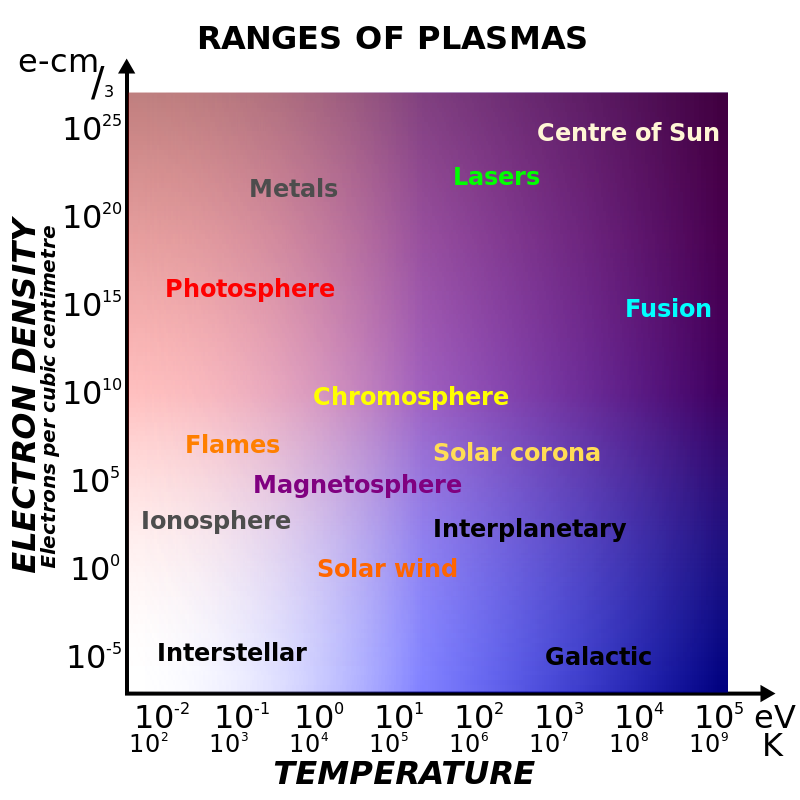
\includegraphics[width=.8\linewidth]{faixaplasma.png}   
\caption{Aumento da densidade para cima, aumento da temperatura para a direita. \cite{figplasma}.}
\end{figure}
		\end{minipage}
	\end{frame}
	\begin{frame}
		\frametitle{Plasma}
		\begin{itemize}
				\item O aquecimento de um gás provoca a dissociação das suas ligações moleculares, convertendo-o em seus átomos constituintes \cite{tokamaks}.
	\item A magnetohidrodinâmica (MHD) é a área da física que estuda a interação mútua entre fluidos condutores e campos eletromagnéticos. 
\end{itemize}

\end{frame}
%fusão
	\section{Fusão}
\begin{frame}
	   \frametitle{Fusão}
	   \framesubtitle{A fusão nuclear é uma fonte promissora de energia para suprir a crescente demanda mundial.}
		\begin{minipage}[H]{.4\textwidth}
		 \begin{itemize}

\item Núcleos de baixa massa se fundem para formar núcleos mais massivos.
\item Após uma reação de fusão, as massas totais são menores do que antes: a massa “ausente” é convertida em energia. \cite{tokamaks}

\end{itemize}
		\end{minipage}
		\hfill
		\begin{minipage}[h]{.45\textwidth}
			\begin{figure}
				\centering
				
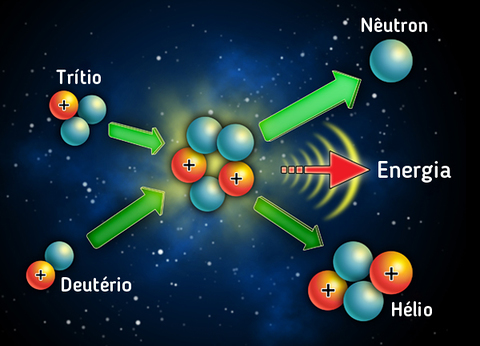
\includegraphics[width=.8\linewidth]{fusaoimage.png}
\caption{Esquema básico da fusão, fonte: todamateria.}   
\end{figure}
		\end{minipage}
	\end{frame}


%tokamak	
\section{Tokamaks}
	\begin{frame}
		\frametitle{Tokamak}
		\framesubtitle{Funcionamento básico}
		\begin{minipage}[h]{.4\textwidth}
		\begin{itemize}
		\item  O Tokamak é um reator experimental de
fusão nuclear.
\item  Serve para estudar plasmas de alta temperatura, que são mantidos confinados por campos magnéticos intensos.
		\end{itemize}
			\end{minipage}
		\hfill
		\begin{minipage}[h]{.55\textwidth}
			\begin{figure}
						\centering
			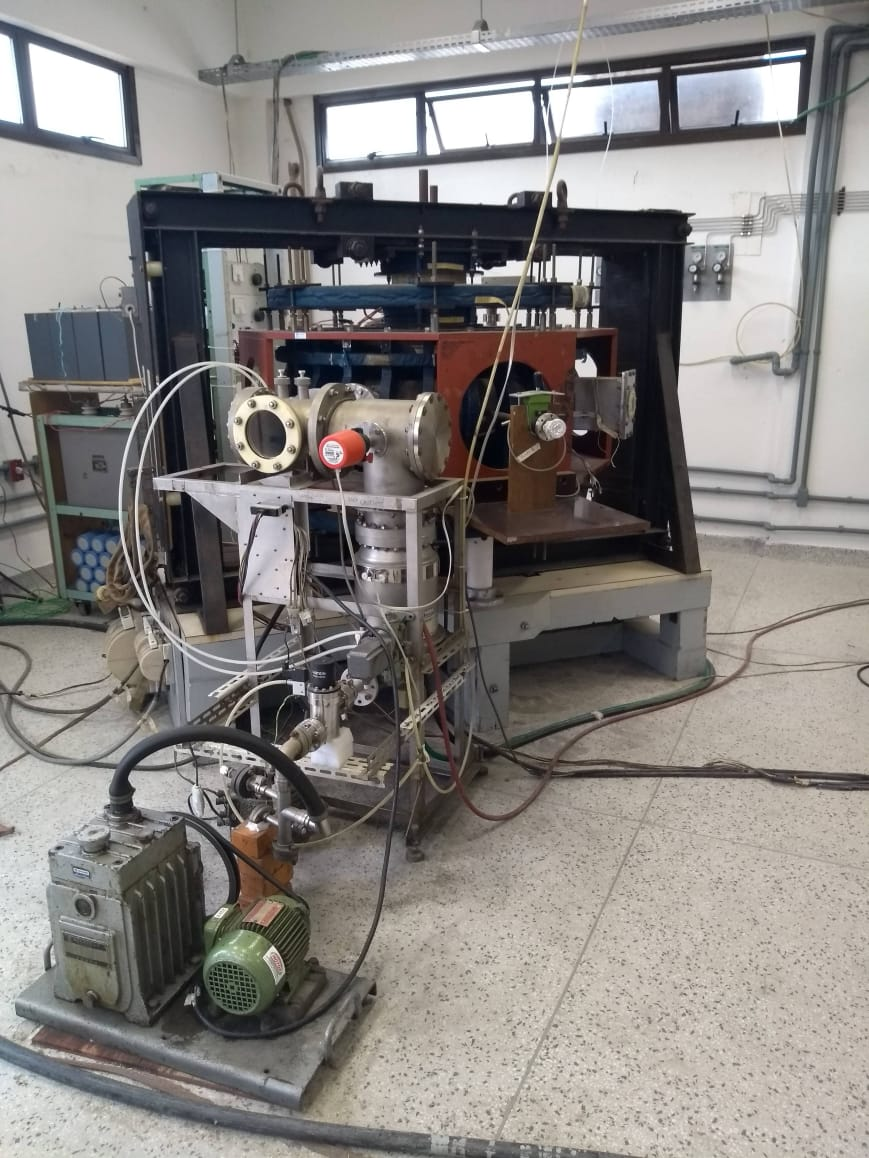
\includegraphics[width=.55\linewidth]{tokamak.jpeg} 
			\caption{Tokamak NOVA-FURG.}
			\end{figure} 	
			\end{minipage}
	\end{frame}	
	
	\begin{frame}
		\frametitle{Tokamak}
			\begin{figure}[H]
				\centering
			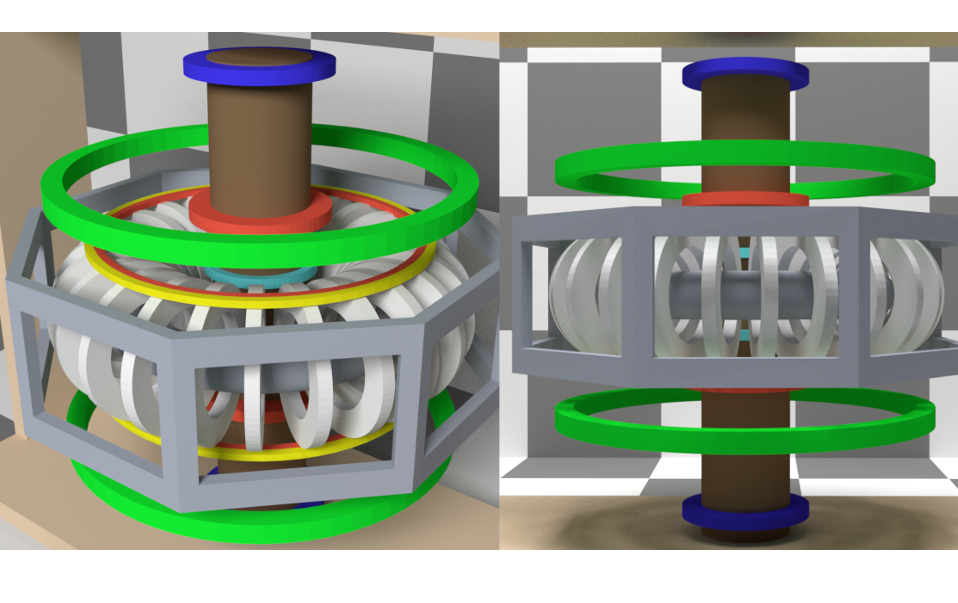
\includegraphics[width=.65\linewidth]{tokamak12.png} 
				\caption{Tokamak NOVA-FURG, modelo feito no Blender.}
		
			\end{figure}	
	\end{frame}

	
	\begin{frame}
		\frametitle{Tokamak}
		\framesubtitle{Fase de breakdown}
\begin{itemize}
\item  A fase de breakdown em um tokamak é dominada por colisões entre elétrons livres e partículas neutras.
\item Acontece um efeito avalanche que rapidamente ioniza o gás transformando-o em plasma.
\item Este processo pode ser estimado por um modelo tipo Townsend \cite{yoo2014ohmic}. %, que assume que, devido à sua maior massa, os íons são estacionários, e os elétrons livres são responsáveis pela

	\begin{figure}[H]
				\centering
			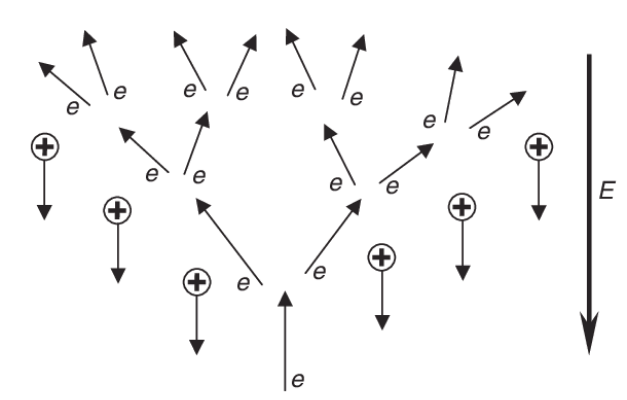
\includegraphics[width=.4\linewidth]{avalanche.png} 
				\caption{Ilustração do breakdown de Townsend \cite{article0}.}
		
			\end{figure}
\end{itemize}

	\end{frame}
	

\section{Desenvolvimento do modelo de dois fluidos}

%---------------------------------------------------------------------------
	%eqs
   \begin{frame}
		\frametitle{Equação de Boltzmann}
		
\begin{equation}
\label{eq: boltsmam}
\frac{\partial f_\alpha(\bm{r},\bm{v},t)}{\partial t} +\bm{v} \nabla f_\alpha(\bm{r},\bm{v},t) + \bm{a} \nabla_v f_\alpha(\bm{r},\bm{v},t) = \bm{C}_\alpha,
\end{equation} 
\begin{equation}
\label{eq: boltzzz}
\frac{\partial f_\alpha(\bm{r},\bm{v},t)}{\partial t} +\bm{v} \bm{\nabla} f_\alpha(\bm{r},\bm{v},t) + \frac{1}{m_\alpha}[\bm{F}_{ext}+\bm{E}_{pl}+\bm{v} \times \bm{B}_{pl}] \cdot \bm{\nabla}_v f_\alpha(\bm{r},\bm{v},t)= \bm{C}_\alpha,
\end{equation}
\begin{itemize}
\item $\bm{C}_\alpha = \sum_\beta \bm{C}_{\alpha \beta}$\{$f_\alpha$, $f_\beta$\} é o operador de colisão.
\item  $f_\alpha(\bm{r},\bm{v},t)$ é a distribuição de velocidades da espécie de partículas $\alpha$.
\item  $\bm{F}_{ext}$ representa a força externa.
\item $\bm{E}_{pl}$ e $\bm{B}_{pl}$ são os campos elétrico e magnético gerados pelo plasma.%causados pela presença e movimento de todas as partículas carregadas dentro do plasma.
\end{itemize}

	\end{frame}
	
   \begin{frame}
\frametitle{Equações de Maxwell}

\begin{itemize}
\item $\bm{E}_{pl}$ e $\bm{B}_{pl}$  devem satisfazer as equações de Maxwell.
\item $\mu_0$ é a permeabilidade magnética do vácuo, $\epsilon_0$ é a constante de permissividade do vácuo com $c$ sendo a velocidade da luz no vácuo. 
\end{itemize}
\begin{equation}
\label{eq: max1}
\bm{\nabla} \cdot \bm{E}_{pl} = \frac{\rho}{\epsilon_0},
\end{equation}
\begin{equation}
\label{eq: max2}
\bm{\nabla} \cdot \bm{B}_{pl} = 0,
\end{equation}
\begin{equation}
\label{eq: max3}
\bm{\nabla} \times \bm{E}_{pl} = -\frac{\partial \bm{B}_{pl}}{\partial t},
\end{equation}
\begin{equation}
\label{eq: max4}
\bm{\nabla} \times \bm{B}_{pl} = \mu_0 (\bm{J} + \epsilon_0 \frac{\partial \bm{E}_{pl}}{\partial t} ).
\end{equation}
\end{frame}

    \begin{frame}
\frametitle{Densidade de carga e Densidade de corrente}
\begin{equation}
\label{eq: rho}
\rho(\bm{r},t) = \sum_\alpha q_\alpha n_\alpha(\bm{r},t) = \sum_\alpha q_\alpha \int_v f_\alpha(\bm{r},\bm{v},t) d^3v,
\end{equation}
$\rho$ é a densidade de carga do plasma. 

\begin{equation}
\label{eq: densidadecorrente}
\bm{J}(\bm{r},t) = \sum_\alpha q_\alpha n_\alpha(\bm{r},t) \bm{u}_\alpha(\bm{r},t) = \sum_\alpha  q_\alpha \int_v \bm{v} f_\alpha(\bm{r},\bm{v},t) d^3v,
\end{equation}
$\bm{J}$ é a densidade de corrente de plasma. 

\end{frame}

    \begin{frame}
			\frametitle{Equação geral dos momentos}
		\framesubtitle{Usando esta equação foi deduzido as equações para os três principais momentos da distribuição de velocidades.}
\begin{equation}
\label{eq: pit12}
\frac{\partial }{\partial t}(n_\alpha(\bm{r},t)<\chi>_\alpha) +\bm{ \nabla} \cdot (n_\alpha(\bm{r},t)<\chi \bm{v} >_\alpha) - n_\alpha(\bm{r},t)<\bm{a} \cdot \bm{\nabla_v} \chi>_\alpha = 
\end{equation}
\begin{equation*}
=[\frac{\delta}{\delta t}(n_\alpha(\bm{r},t)<\chi>_\alpha)].
\end{equation*}
\end{frame}	
	
	\begin{frame}
		\frametitle{Simplificações}
		\begin{itemize}
		\item As densidades de correte poloidais, $J_r$ e $J_z$, são assumidas como iguais 0.
		\item  Assumiremos que o plasma é composto por um fluido de elétrons e um único fluido
de íons. 
		\item Ambos incompressíveis, $\bm{\nabla} \cdot \bm{u}_{\alpha} = 0$.  
		\item Fluidos ideais que não possuem viscosidade. %$\mathbb{P}_{\alpha} = p_{\alpha}$. 
		\item Adiabático $\bm{\nabla} \bm{q}_{\alpha} = 0$, $\bm{q}_\alpha$ é o vetor fluxo de calor \cite[pg. 181]{bittencourt}. %, ou seja, com escalas de tempo suficientemente curtas para que não haja difusão de calor, portanto o processo sera considerado adiabático e o 
			\item Transporte de energia é predominantemente convectivo. %Convecção é a transferência de energia térmica pelo movimento de moléculas de uma parte do material para outra. À medida que aumenta o movimento dos fluidos, ocorre a transferência de calor convectiva. A presença de maior movimento do fluido aumenta a transferência de calor entre a superfície do sólido e o fluido. Existem dois tipos de transferência de calor convectiva: Convecção natural: quando o movimento do fluido é causado por forças de empuxo que resultam das variações de densidade devido a variações de temperatura no fluido. Convecção forçada: quando o fluido é forçado a fluir sobre a superfície por fonte externa, como ventiladores e bombas, criando uma corrente de convecção induzida artificialmente. Fluxo interno e externo também podem classifica a convecção. Fluxo interno ocorre quando o fluido é delimitada por uma fronteira sólida, tais como o fluxo através de um tubo. Um fluxo externo ocorre quando o fluido se estende indefinidamente, sem encontrar uma superfície sólida. Ambas as convecções, natural ou forçada, pode ser interna ou externa, porque são independentes uns dos outros.
				\end{itemize}
		
		\end{frame}	
		
	\begin{frame}
		\frametitle{Simplificações}
		\begin{itemize}
	 
		\item Assumimos também que o plasma é quase neutro $n_e = n_i = n$ onde $n$ é a densidade de plasma. 
		%\item Durante a fase de \textit{breakdown} $n_e$ cresce exponencialmente \cite[pg. 52]{kim2013physics}, por consequência, $n$ também cresce exponencialmente. 
		\item Para melhorar a estabilidade numérica, vamos considerar o fluxo total de partículas como sendo composto por um termo convectivo e um difusivo, isto é, $\bm{\Gamma}=n\bm{u}_{\alpha}-D_{\alpha} \bm{\nabla} n$ com $D_e = D_i = D$ sendo o coeficiente de difusão de partículas \cite[pg. 52]{kim2013physics}, \cite[cap 7]{thermalplasmas}.
		\item Admitimos também que o gás neutro está em repouso e à temperatura ambiente.
		\end{itemize}
		
		\end{frame}	
		
		\begin{frame}
		\frametitle{Simplificações}
		\begin{itemize}
		\item  Definimos um termo de fonte de partículas que explique o número de partículas em vez da massa de partículas: $\zeta_\alpha = S_\alpha / m_\alpha$. 
		\item Para um plasma ionizado, podemos dizer que 
		$$\zeta_e = \zeta_i = \zeta = n(\nu_{ion} - \nu_{loss}).$$ 
\item Assumiremos que $$\nu_{ion} = \alpha_T u_e = \alpha_T J / (ne),$$ e $$\nu_{loss} = \frac{u_{e, ||}}{L_{\mathrm{eff}} }= e |\bm{B}| n \big( \bm{J} \cdot \bm{B}  \big).$$ 
\item $\alpha_T$ é o primeiro coeficiente de Townsend.

\item $L_\mathrm{eff}$ é a distância média percorrida pelo elétron antes de se chocar com a parede.
\item $u_{e, ||}$ é a velocidade de deriva.
		\end{itemize}
		\end{frame}	
	\begin{frame}
		\frametitle{Sistema de equações}
		Então o modelo escrito em termos da densidade de corrente ($\bm{J}_\alpha=\bm{u}_\alpha \rho_\alpha$) fica
\begin{equation}
\frac{\partial n}{\partial t} = \bm{\nabla} \cdot \bm{J}+\nu_{ion} - \nu_{loss}+D\nabla^2n,
\end{equation}

\begin{equation}
\label{momenteletrico} 
\frac{\partial \bm{J}}{\partial t} =  \frac{ne^2}{m_e} \bm{E} -\bm{J}(\nu_{in}+\nu_{en}+\nu_{ion}-\nu_{loss}) -\frac{e}{m_e}\bm{J} \times \bm{B}+\frac{e}{m_e}\bm{\nabla} p_e,
\end{equation}

\begin{equation}
\frac{\partial p_e}{\partial t} = \frac{3}{2}(1+\frac{2 \nu_{en} + \nu_{ion} - \nu_{loss}}{2\nu_{ei}})\eta J^2  -\frac{2ne^2}{m_i} \eta (p_e-p_i),
\end{equation}

\begin{equation}
\frac{\partial p_i}{\partial t} = \frac{2ne^2}{m_i}\eta(p_e-p_i).
\end{equation}

\end{frame}



\section{Superfícies de fluxo magnético poloidal}
%\noindent Uma superfície continua dada $S$ com $\bm{n}$ normal é uma superfície de fluxo de um campo vetorial suave $\bm{B}$ quando
%\begin{equation}
%\bm{B} \cdot \bm{n}= 0 
%\end{equation}
%em todo os pontos do $S$. Em outras palavras, o campo magnético não atravessa a superfície $S$ em nenhum lugar, ou seja, o fluxo magnético que atravessa $S$ é zero. É então possível definir uma função de fluxo escalar $f$ tal que seu valor seja constante na superfície $S$ e
%\begin{equation}
%\bm{B} \cdot \bm{\nabla} f = 0.
%\end{equation}
\begin{frame}		
\frametitle{Render bobinas tokamak NOVA-FURG}
\begin{figure}[H]
\centering
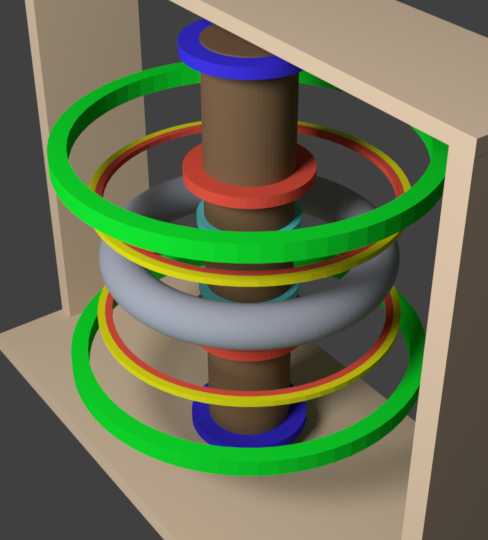
\includegraphics[width=.37\linewidth]{bob2.png}  
\caption{Bobinas tokamak NOVA-FURG - Modelo criado no Blender.}
\end{figure}
\end{frame}

\begin{frame}		
\frametitle{ Superfícies de fluxo magnético poloidal }
\begin{itemize}
\item Superfícies de fluxo do campo magnético poloidal $B_{ext}$, geradas pelas bobinas do tokamak NOVA-FURG.
\item Para obtê-las, monta-se uma tabela de Green para o campo magnético gerado por cada bobina com uma corrente unitária \cite{MagneticControl}.
\item Definiu-se a distribuição de campo magnético $\bm{\Psi}(\bm{r})$ como a soma dos valores de cada tabela de Green, em cada $\bm{r}$, multiplicados pela corrente que passa pela mesma.
\end{itemize}
\end{frame}


\begin{frame}		
\frametitle{ Superfícies de fluxo magnético poloidal }
\framesubtitle{Figuras das superfícies de fluxo magnético poloidal gerado pelas bobinas do tokamak NOVA-FURG}

		\begin{figure}[H]
\centering %Superfícies de fluxo magnético poloidal geradas pelas bobinas do tokamak NOVA-FURG - Imagem feita no MATLAB, com valores de corrente ilustrativos.  
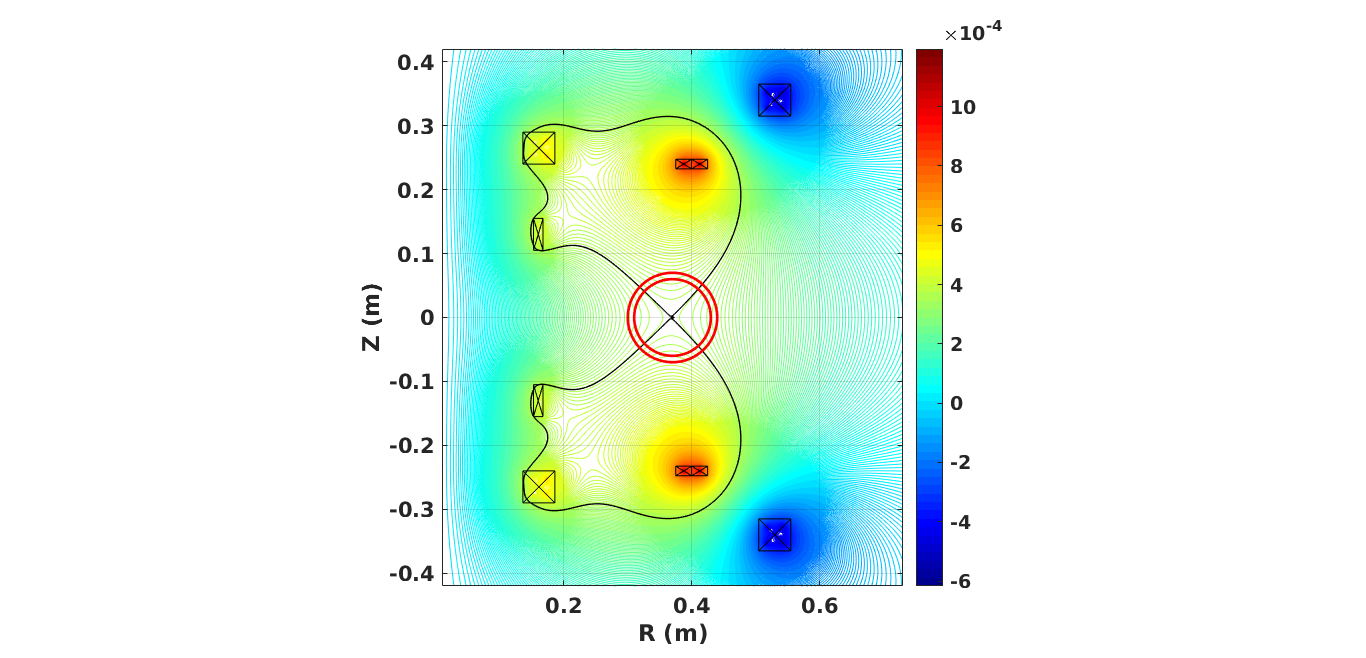
\includegraphics[scale=0.3]{campo001-2.png} 
\caption{Em preto a superfície de fluxo magnético poloidal correspondente a $\bm{\Psi}(\bm{r}_{xp})$, onde $\bm{r}_{xp}=(0.37,0)$ é o ponto-X (T$\cdot m^2$).}
\label{fig: equipotenc}
\end{figure}

\end{frame}

\begin{frame}		
\frametitle{ Superfícies de fluxo magnético poloidal }
\framesubtitle{Figuras das superfícies de fluxo magnético poloidal gerado pelas bobinas do tokamak NOVA-FURG}

	\begin{figure}[H]
\centering
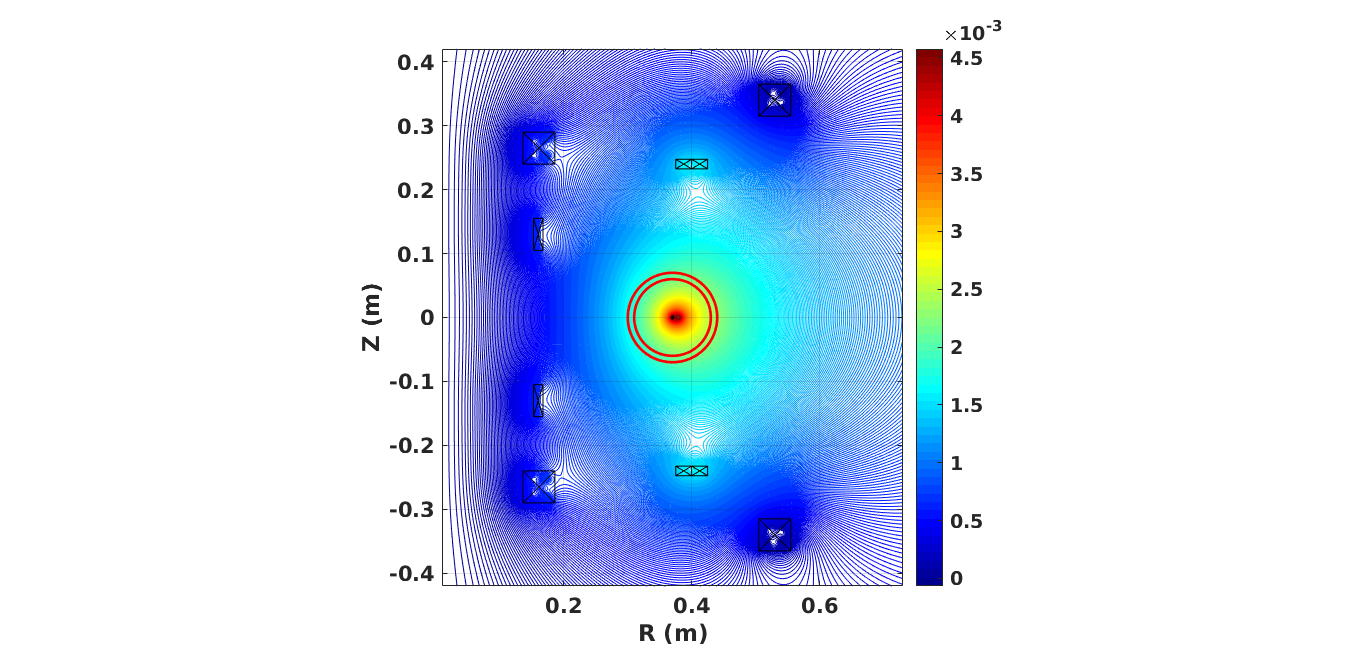
\includegraphics[scale=0.3]{campo002-2.png} 
\caption{Com o campo magnético gerado pela corrente de plasma (T$\cdot m^2$).}
\label{fig: equipotenc2}
\end{figure}

\end{frame}
\section{Equações dos campos eletromagnéticos}

\begin{frame}		
\frametitle{Componente externo e de plasma do campo eletromagnético}
\begin{itemize}
\item Separando os campos em um componente gerado pelas correntes que fluem em bobinas fora do plasma e outro causado pelo plasma. \cite[cap. 2]{MagneticControl}.
$$\bm{E} = \bm{E}_{ext} + \bm{E}_{pl}$$   
$$\bm{B} = \bm{B}_{ext} + \bm{B}_{pl}$$
\item O campo magnético aplicado externamente é produzido por um conjunto de bobinas específicas fora do plasma e possui componentes poloidais e toroidais. 
\item  O campo toroidal tem uma dependência $1 / R$.
\item O campo poloidal tem um padrão quadrupolo.
\end{itemize}
\begin{equation}
\label{Bext}
\bm{B}_{ext}=\bm{B}_{pol}^{quadrupole}+\frac{R_0B_0}{R}\hat{e}_{\phi} .
\end{equation}
\end{frame}


\begin{frame}		
\frametitle{Componente externo e de plasma do campo eletromagnético}
\framesubtitle{Expressão para o campo elétrico externo}
\begin{itemize}
\item O campo elétrico aplicado externamente é produzido pelo solenoide central do tokamak, que induz uma voltagem de loop toroidal, $V_{loop}$. 
\end{itemize}
O campo elétrico externo é então dado por
\begin{equation}
\label{Eext}
\bm{E}_{ext} = \frac{V_{loop}}{2\pi R} \hat{e}_{\phi} .
\end{equation}
O campo eletromagnético gerado pelo plasma é calculado via
\begin{equation}
\nabla^2 \bm{A}_{pl}=-\mu_0\bm{J} 
\end{equation}
\end{frame}


\begin{frame}		
\frametitle{Componente externo e de plasma do campo eletromagnético}
\framesubtitle{Expressões para o calculo do campo elétrico e magnético gerado pelo plasma}
\begin{itemize}
\item $A_{pl}$ é o vetor de potencial magnético devido ao plasma.
\item Os campos eletromagnéticos externos $\bm{E}_{ext}$ e $\bm{B}_{ext}$ são formados antes do plasma e se mantêm constantes.
\end{itemize}
 O campo eletromagnético então segue de
\begin{equation}
\bm{B}_{pl} = \bm{\nabla} \times \bm{A}_{pl},
\end{equation}
\begin{equation}
\bm{E}_{pl}=-\frac{\partial \bm{A}_{pl}}{\partial t} .
\end{equation}

\end{frame}


\section{Condições iniciais e de contorno}

\begin{frame}		
\frametitle{Condições iniciais}
\framesubtitle{ }
\begin{itemize}
\item $Te_0$ é a temperatura inicial de elétrons.
\item $\nu_{eff}=\nu_{ei} + \nu_{en} + \nu_{in} + \nu_{loss}$ é a frequência efetiva de colisão de elétrons.
%\item as equações para calcular $\nu_{eff}$ estão em \ref{Townsend}.
\item $\nu_{ei}$ é calculado no início e se mantêm constante. 
\item $\nu_{en}$ é atualizado a cada passo temporal por $\nu_{en}=7.89 \times 10^{11} k_B T_{e0}(n_g-n)$. \item $n_g$ é a densidade de partículas neutras inicial 
\item $e$ é a carga elétrica elementar. 
\item $n_0$ é a densidade inicial de partículas.
\item  $p_e$ e $p_i$ são respectivamente os escalares iniciais de pressão cinética eletrônica e iônica. 
\item Só existe campo elétrico na direção toroidal $\phi$ então, $\bm{E}_{ext} = \frac{V_{loop}}{2\pi R} \hat{e}_{\phi} $, eq. \ref{Eext}. 
\end{itemize}

\end{frame}
\begin{frame}		
\frametitle{Condições iniciais}
\framesubtitle{ } 
\begin{itemize}

\item Na borda do domínio temos fixadas as mesmas condições que na condição inicial do interior.
\item No tempo zero, quando não estamos usando a aproximação pela gaussiana eq. \ref{gaussiana} sempre temos $\nu_{in} = \nu_{loss} = 0$.
\item A condição inicial da resistividade depende de $T_{e_0}$ e $n_0$. %código \ref{codigosresitivit} no apêndice \ref{codigos}.
$$n = n_0,$$
$$J_{\phi}= \frac{n_0 e^2 }{m_e \nu_{eff}} E_{ext,\phi},$$
$$p_e=n_0 k_B T_{e_0},$$
$$p_i=n_0 k_B T_{i_0}. $$
\end{itemize}
\end{frame}


\section{Resultados código explícito no tempo}

\begin{frame}
		\frametitle{Coordenadas}
		\framesubtitle{Mudança pensada para facilitar a introdução das condições de contorno}
	
		\begin{figure}[H]
			\centering
			
			\begin{subfigure}{0.45\textwidth}
				\centering
				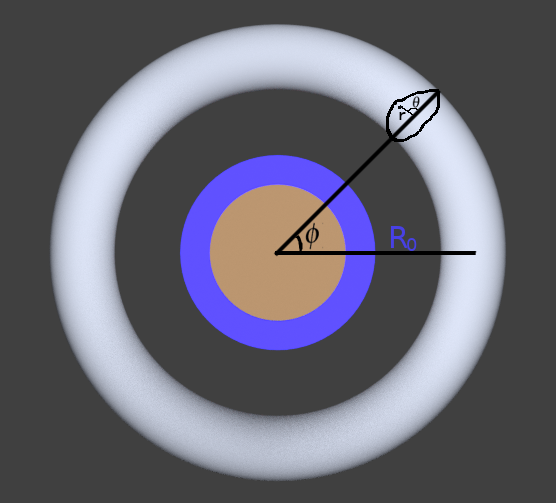
\includegraphics[width=.9\linewidth]{pseudotoridal1.png}
				\caption{Coordenadas pseudo-toroidais.} 
			\end{subfigure}
			\hfill
			\begin{subfigure}{0.45\textwidth}
				\centering
				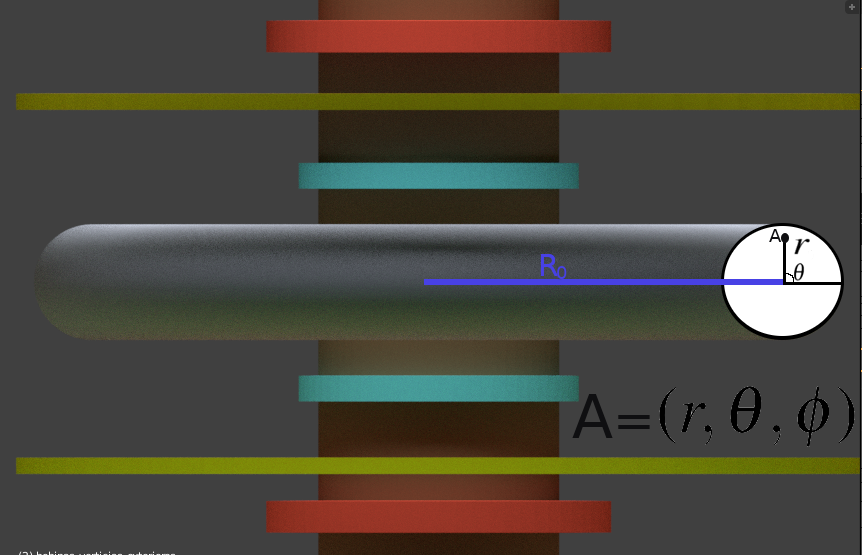
\includegraphics[width=.9\linewidth]{pseudotoridal2.png}
				\caption{O ponto $A$ representado em coordenadas pseudo-toroidais.} 
			\end{subfigure}                                                   
			
		\end{figure}	
	\end{frame}
		   \begin{frame}
			\frametitle{Pseudo-toroidais}
		%\framesubtitle{}
	\begin{equation}
\label{rX}
X(r,\theta,\phi) = (R_0+r \cos(\theta)) \cos(\phi),
\end{equation}
\begin{equation}
\label{rY}
Y(r,\theta,\phi) = (R_0+r \cos(\theta)) \sin(\phi),
\end{equation}
\begin{equation}
\label{rZ}
Z(r,\theta,\phi) = -r \sin(\theta).
\end{equation}
Onde os valores possíveis para cada coordenada são
\begin{equation}
0 \leq \phi < 2 \pi,
\end{equation}
\begin{equation}
0 \leq \theta < 2 \pi,
\end{equation}
\begin{equation}
\label{maxr}
0 < r \leq a_0,
\end{equation}
	\end{frame}
	   \begin{frame}
			\frametitle{Pseudo-toroidais}
	%	\framesubtitle{Pseudo-toroidais}
\begin{equation}
ds=|d\bm{r_p}| = \sqrt{[dr]^2+  [r d\theta ]^2+[(R_0+r \cos(\theta)) d\phi ]^2},
\end{equation}
\begin{equation}
\bm{\nabla} \varphi = \dfrac{\partial \varphi}{\partial r}  \hat{e}_r + \left(\frac{1}{r}\dfrac{\partial \varphi}{\partial \theta} \right) \hat{e}_\theta + \left( \left[ \frac{1}{ R_0 + r \cos(\theta)}\right] \dfrac{\partial \varphi}{\partial \phi}\right) \hat{e}_\phi,
\end{equation}
\begin{equation}
\bm{\nabla} \cdot \bm{u} = \frac{1}{r R_0 + r^2 \cos(\theta)} \left[ \dfrac{\partial}{\partial r} \Big[u_r \big(r R_0 + r^2 \cos(\theta)\big)\Big] + \dfrac{\partial}{\partial \theta}\Big[ u_\theta \big( R_0 + r \cos(\theta) \big) \Big] +  \dfrac{\partial }{\partial \phi}\big( u_\phi  r \big) \right],
\end{equation}

	\end{frame}
		   \begin{frame}
			\frametitle{Pseudo-toroidais}
		%\framesubtitle{Pseudo-toroidais}
\begin{equation}
\nabla^2 f = \dfrac{\partial f}{\partial r}  \hat{e}_r + \left(\frac{1}{r}\dfrac{\partial f}{\partial \theta} \right) \cdot \hat{e}_\theta + \left( \left[ \frac{1}{ R_0 + r \cos(\theta)}\right] \dfrac{\partial f}{\partial \phi}\right)  \hat{e}_\phi,
\end{equation}
\begin{equation}
\bm{\nabla} \times \bm{u} = \frac{1}{r R_0 + r^2 \cos(\theta)} \left[ \dfrac{\partial }{\partial \theta} \Big[ u_\phi \big(R_0 + r \cos(\theta)\big)\Big] - \dfrac{\partial }{\partial \phi} \big( u_\theta r \big) \right] \hat{e}_r+
\end{equation}
\begin{equation*}
\frac{1}{R_0 + r \cos(\theta)} \left[ \dfrac{\partial u_r}{\partial \phi} - \dfrac{\partial }{\partial r} \Big[ u_\phi  \big( R_0 + r \cos(\theta) \big) \Big] \right] \hat{e}_\theta+\frac{1}{r} \left[ \dfrac{\partial }{\partial r}\big( u_\theta  r\big) - \dfrac{\partial u_r}{\partial \theta}  \right] \hat{e}_\phi.
\end{equation*}
	\end{frame}

	\begin{frame}		
\frametitle{Gaussiana}
\begin{itemize}
\item $x_0$ é quando o ponto onde o campo magnético é zero está deslocado do centro da geometria na direção x.
\item $s_0$ e $\sigma$ são constantes para ajustar a curva.
\end{itemize}
\begin{equation}
\label{gaussiana}
s = \nu_{ion} - \nu_{loss} = s_0 e^{-\frac{ (x+x_0)^2+y^2 }{\sigma}} .
\end{equation} 
\begin{figure}[H]
\centering
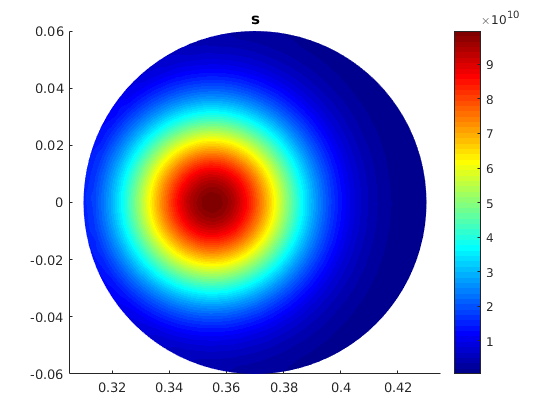
\includegraphics[scale=0.3]{../SImulacao_breakdown/PDE/sB.png} 
\caption{Gaussiana usada para modelar o termo de fonte de partículas $\nu_{ion} - \nu_{loss}$ ($s^{-1}$) ( $s_0=10^{10}$, $x_0=0.015$\ m e $\sigma=0.001$).}
\label{grafgaussiana}
\end{figure}
\end{frame}	
	
	\begin{frame}
		\frametitle{Primeiro resultado}
		\framesubtitle{NOVA-FURG}
Alguns resultados iniciais usando o código explícito e considerando nulos os campos internos elétricos e magnéticos. 
	\end{frame}
	\begin{frame}
		\frametitle{Abordagem explícita}
		%\framesubtitle{NOVA-FURG}
\begin{figure}[H]
\centering
\includegraphics[scale=0.3]{../SImulacao_breakdown/Adaptacao_nova/Jphi(:,:,3).png} 
\includegraphics[scale=0.3]{../SImulacao_breakdown/Adaptacao_nova/pion(:,:,3).png}  
\caption{Densidade de plasma ($m^{-1}$), componente toroidal da densidade de corrente de plasma ($A/m^2$), pressões eletrônica e iônica ($Pa$) ($dt=10^{-6}$\ s, $N_g = 65$ e $t=3dt$).}
\label{fig:simul1} 
\end{figure}
			
	\end{frame}
	\begin{frame}
		\frametitle{Abordagem explícita}

\begin{figure}[H]
\label{simul04}
\begin{center}
\includegraphics[scale=0.3]{../SImulacao_breakdown/Adaptacao_nova/Jphi(:,:,83).png} 
\includegraphics[scale=0.3]{../SImulacao_breakdown/Adaptacao_nova/pion(:,:,83).png}  
\caption{Densidade de plasma ($m^{-1}$), componente toroidal da densidade de corrente de plasma ($A/m^2$), pressões eletrônica e iônica ($Pa$) ($dt=10^{-6}$\ s, $N_g = 65$ e $t=83dt$).}
\end{center}
\end{figure}
	\end{frame}
	\begin{frame}
		\frametitle{Abordagem explícita}

\begin{figure}[H]
\label{simul4}
\begin{center}
\includegraphics[scale=0.3]{../SImulacao_breakdown/Adaptacao_nova/Jphi(:,:,123).png}
\includegraphics[scale=0.3]{../SImulacao_breakdown/Adaptacao_nova/pion(:,:,123).png}   
\caption{Densidade de plasma ($m^{-1}$), componente toroidal da densidade de corrente de plasma ($A/m^2$), pressões eletrônica e iônica ($Pa$) ($dt=10^{-6}$\ s, $N_g = 65$ e $t=523dt$).}
\end{center}
\end{figure}
	\end{frame}
	\begin{frame}
		\frametitle{Abordagem explícita}

\begin{figure}[H]
\label{simul8}
\begin{center}
\includegraphics[scale=0.3]{../SImulacao_breakdown/Adaptacao_nova/Jphi(:,:,203).png}  
\includegraphics[scale=0.3]{../SImulacao_breakdown/Adaptacao_nova/pion(:,:,203).png} 
\caption{Densidade de plasma ($m^{-1}$), componente toroidal da densidade de corrente de plasma ($A/m^2$), pressões eletrônica e iônica ($Pa$) ($dt=10^{-6}$\ s, $N_g = 65$ e $t=203dt$).}
\end{center}
\end{figure}
	\end{frame}
	\begin{frame}
		\frametitle{Abordagem explícita}


\begin{figure}[H]
\begin{center}
\includegraphics[scale=0.3]{../SImulacao_breakdown/Adaptacao_nova/Jphi(:,:,283).png}  
\includegraphics[scale=0.3]{../SImulacao_breakdown/Adaptacao_nova/pion(:,:,283).png}  
\caption{Densidade de plasma ($m^{-1}$), componente toroidal da densidade de corrente de plasma ($A/m^2$), pressões eletrônica e iônica ($Pa$) ($dt=10^{-6}$\ s, $N_g = 65$ e $t=283dt$).}
\end{center}
\end{figure}
	\end{frame}
	\begin{frame}
		\frametitle{Abordagem explícita}


\begin{figure}[H]
\label{simul15}
\begin{center}
\includegraphics[scale=0.3]{../SImulacao_breakdown/Adaptacao_nova/Jphi(:,:,363).png} 
\includegraphics[scale=0.3]{../SImulacao_breakdown/Adaptacao_nova/pion(:,:,363).png}  
\caption{Densidade de plasma ($m^{-1}$), componente toroidal da densidade de corrente de plasma ($A/m^2$), pressões eletrônica e iônica ($Pa$) ($dt=10^{-6}$\ s, $N_g = 65$ e $t=363dt$).}
\end{center}
\end{figure}
	\end{frame}
	\begin{frame}
		\frametitle{Abordagem explícita}


\begin{figure}[H]
\label{simul19}
\begin{center}
\includegraphics[scale=0.3]{../SImulacao_breakdown/Adaptacao_nova/Jphi(:,:,443).png}  
\includegraphics[scale=0.3]{../SImulacao_breakdown/Adaptacao_nova/pion(:,:,443).png}  
\caption{Densidade de plasma ($m^{-1}$), componente toroidal da densidade de corrente de plasma ($A/m^2$), pressões eletrônica e iônica ($Pa$) ($dt=10^{-6}$\ s, $N_g = 65$ e $t=443dt$).}
\end{center}
\end{figure}
	\end{frame}
	\begin{frame}
		\frametitle{Abordagem explícita}


\begin{figure}[H]
\label{simul23}
\begin{center}
\includegraphics[scale=0.3]{../SImulacao_breakdown/Adaptacao_nova/Jphi(:,:,523).png} 
\includegraphics[scale=0.3]{../SImulacao_breakdown/Adaptacao_nova/pion(:,:,523).png}  
\caption{Densidade de plasma ($m^{-1}$), componente toroidal da densidade de corrente de plasma ($A/m^2$), pressões eletrônica e iônica ($Pa$) ($dt=10^{-6}$\ s, $N_g = 65$ e $t=523dt$).}
\end{center}
\end{figure}
	\end{frame}
	\begin{frame}
		\frametitle{Abordagem explícita}


\begin{figure}[H]
\centering
\includegraphics[scale=0.3]{../SImulacao_breakdown/Adaptacao_nova/Jphi(:,:,563).png} 
\includegraphics[scale=0.3]{../SImulacao_breakdown/Adaptacao_nova/pion(:,:,563).png}  
\caption{Densidade de plasma ($m^{-1}$), componente toroidal da densidade de corrente de plasma ($A/m^2$), pressões eletrônica e iônica ($Pa$) ($dt=10^{-6}$\ s, $N_g = 65$ e $t=563dt$).}
\label{fig:simul26} 
\end{figure}	
	
	\end{frame}

\section{PDE solver no MATLAB}
\begin{frame}
\frametitle{Introdução ao PDE solver}
\framesubtitle{Sistemas no formato matricial apenas em cartesianas}
\begin{itemize}
\item O sistema a ser resolvido pelo PDE solver deve estar no formato 

\begin{equation}
\bm{m} \frac{\partial^2 \bm{u}}{\partial t^2} + \bm{d} \frac{\partial \bm{u}}{\partial t} - \bm{\nabla} \cdot \left( \bm{c} \bm{\nabla} \bm{u} \right) + \bm{a}\bm{u} = \bm{f}.
\label{sistemapde}
\end{equation} 
\item Neste trabalho $\bm{u}=[n, J_\phi, p_e, p_e]$.
\item O domínio será circular, com raio $a_0$ e deslocado em $R_0$ a direita da origem. 
\item O PDE Solver aceita apenas problemas em cartesianas. 
\item O sistema matricial foi reescrito em  cartesianas.
\end{itemize}
\end{frame}
\begin{frame}
\frametitle{Formato Matricial}
\framesubtitle{Sistema implementado no PDE solver}
\begin{displaymath}
\left(\begin{array}{c}
x \\
0\\
1\\
1
\end{array}\right)
\left(\begin{array}{c}
\frac{\partial n}{\partial t}\\
\frac{\partial J_\phi}{\partial t}\\
\frac{\partial p_e}{\partial t}\\
\frac{\partial p_i}{\partial t}
\end{array}\right) - \bm{\nabla} \cdot \left( \left(\begin{array}{c}
x D\\
0\\
0\\
0
\end{array}\right) \bm{\nabla} \left(\begin{array}{c}
n\\
J_\phi\\
p_e\\
p_i
\end{array}\right) \right) + \left(\begin{array}{c}
0\\
(\nu_{in}+\nu_{en}+\nu_{ion}-\nu_{loss})\\
\frac{2ne^2}{m_i} \eta\\
\frac{2ne^2}{m_i} \eta
\end{array}\right)\left(\begin{array}{c}
n\\
J_\phi\\
p_e\\
p_i
\end{array}\right) =
\end{displaymath}
\begin{displaymath}
= \left(\begin{array}{c}
x ( \nu_{ion} - \nu_{loss} )\\
\frac{ne^2}{m_e} \bm{E} \\
\frac{3}{2}(1+\frac{2 \nu_{en} + \nu_{ion} - \nu_{loss}}{2\nu_{ei}})\eta |J_\phi|  +\frac{2ne^2}{m_i} \eta p_e\\
\frac{2ne^2}{m_i}\eta p_e
\end{array}\right).
\end{displaymath}

\end{frame}	
	
	%resultados
	
	
	
\section{Aproximação da taxa de ionização menos perda por uma gaussiana}
   
\begin{frame}
		\frametitle{Malha PDE solver}
			
	\begin{figure}[H]
	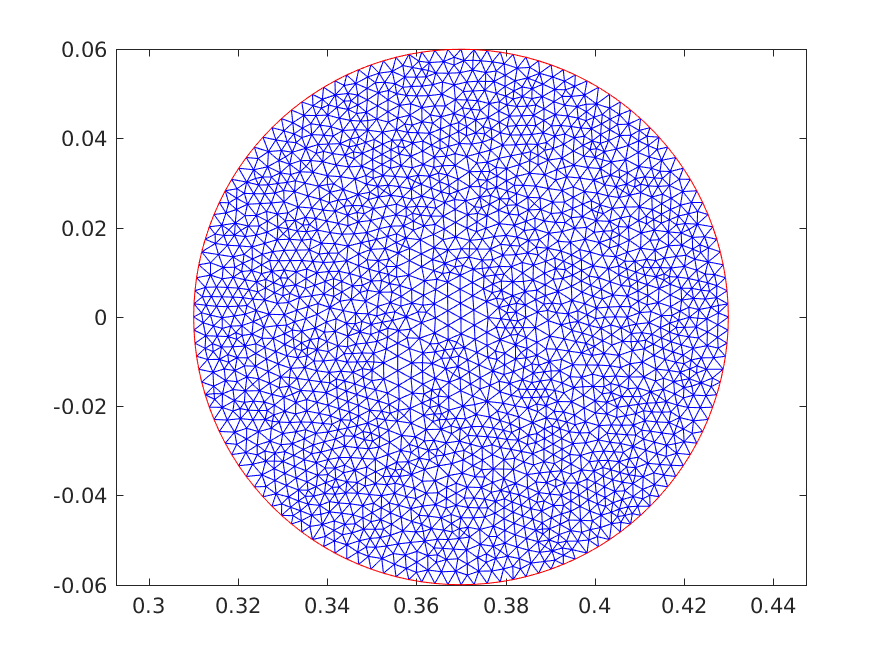
\includegraphics[width=.5\linewidth]{../SImulacao_breakdown/PDE/malha.png}  
	\caption{Mesh triangular com $H_{max}=0.006$.} 	
			\centering
			\end{figure}	
	\end{frame}
	
\begin{frame}
\frametitle{Aproximação da taxa de ionização menos perda por uma gaussiana}
\begin{figure}[H]
\begin{subfigure}{0.43\textwidth}
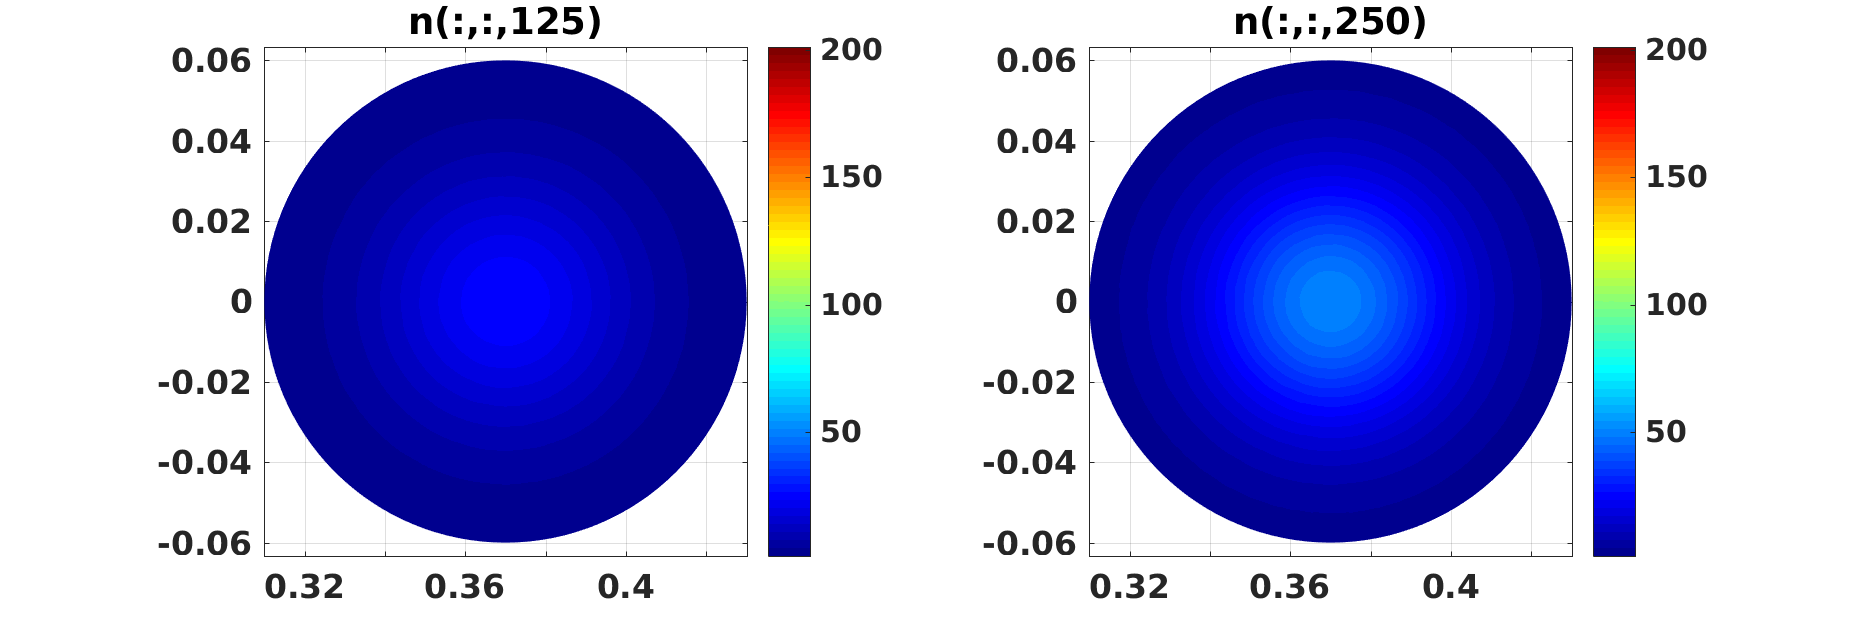
\includegraphics[scale=0.24]{../SImulacao_breakdown/PDE/ntod1B6.png}  
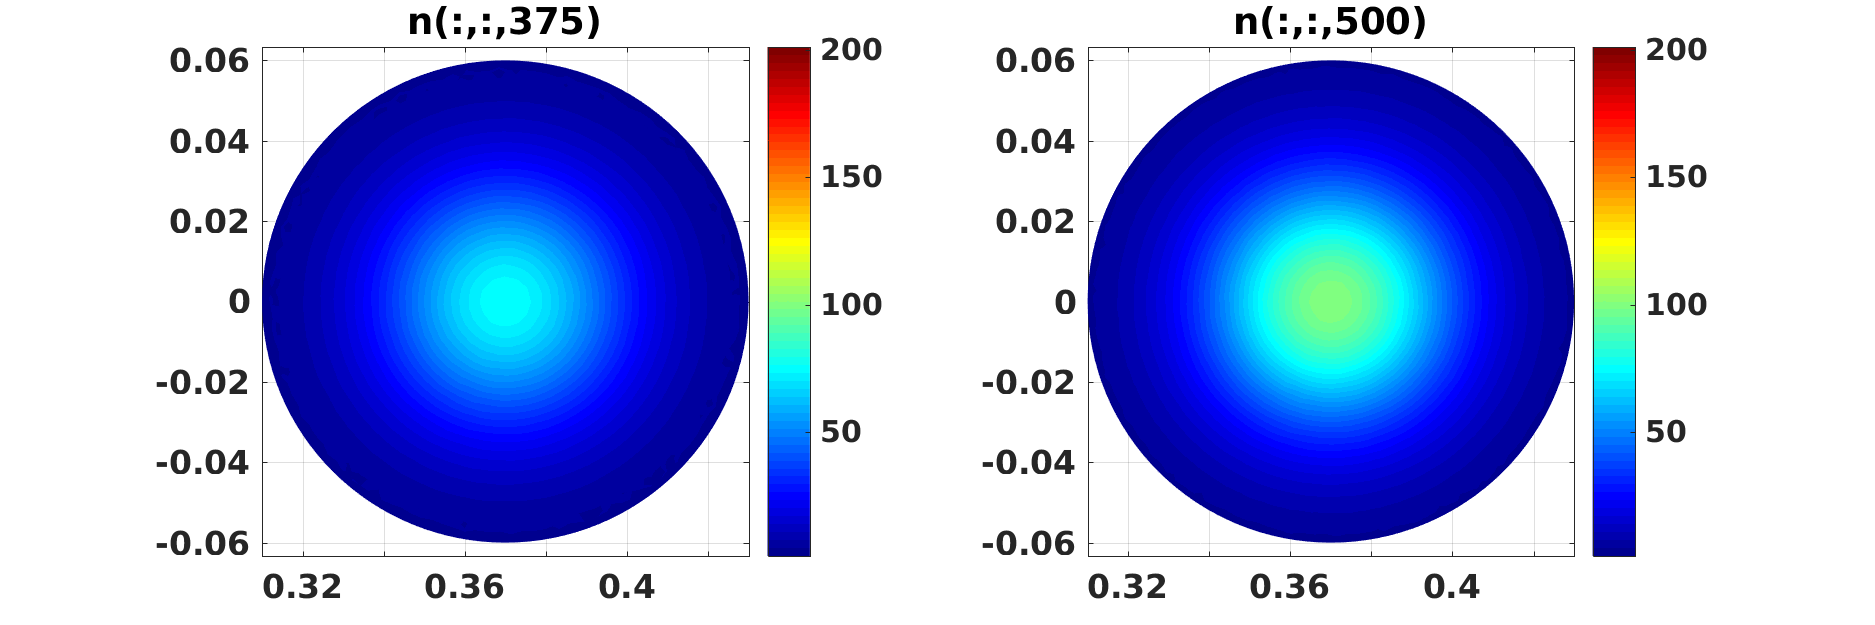
\includegraphics[scale=0.24]{../SImulacao_breakdown/PDE/ntod2B6.png} 
\end{subfigure}
\begin{subfigure}{0.43\textwidth}
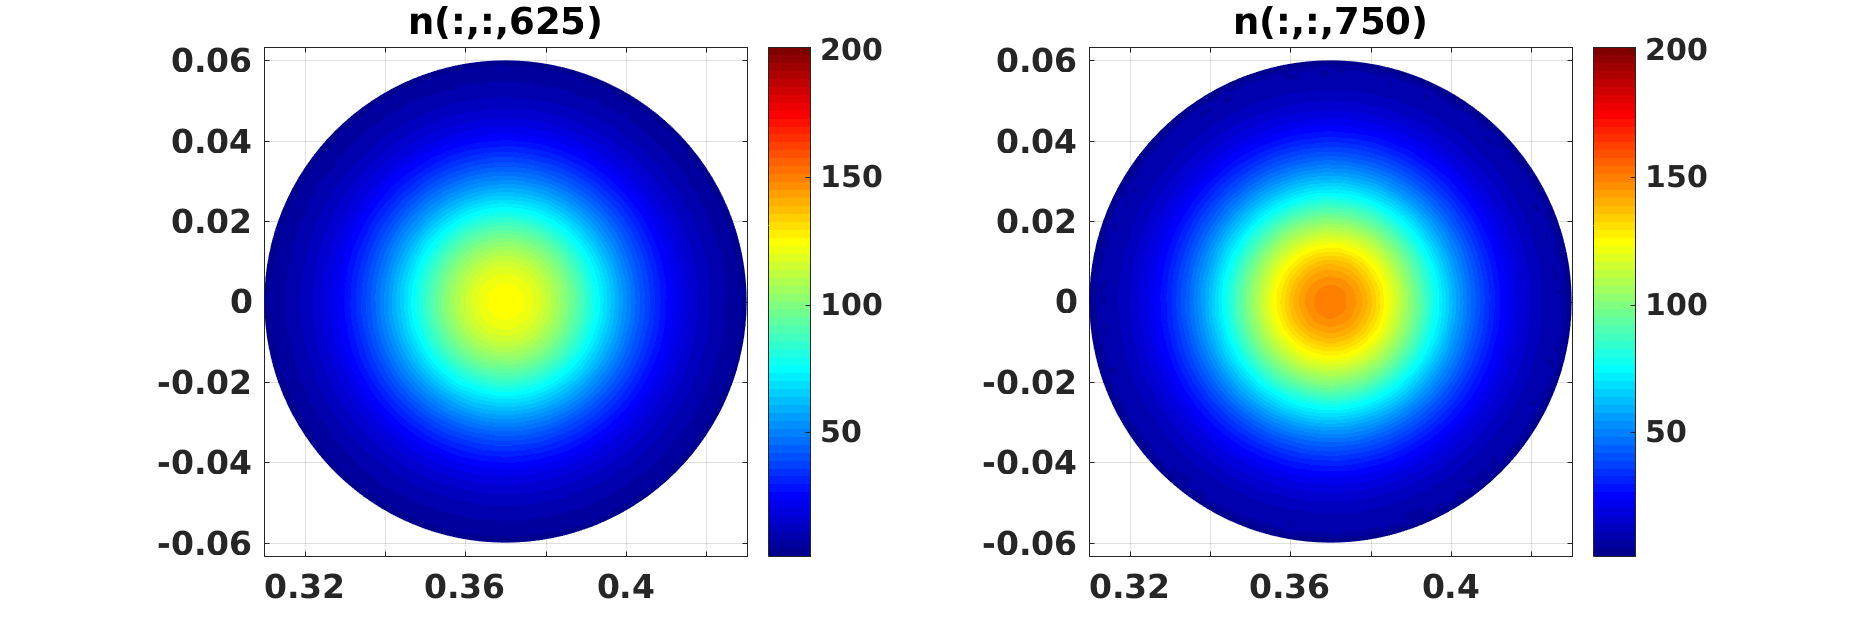
\includegraphics[scale=0.24]{../SImulacao_breakdown/PDE/ntod3B6.png} 
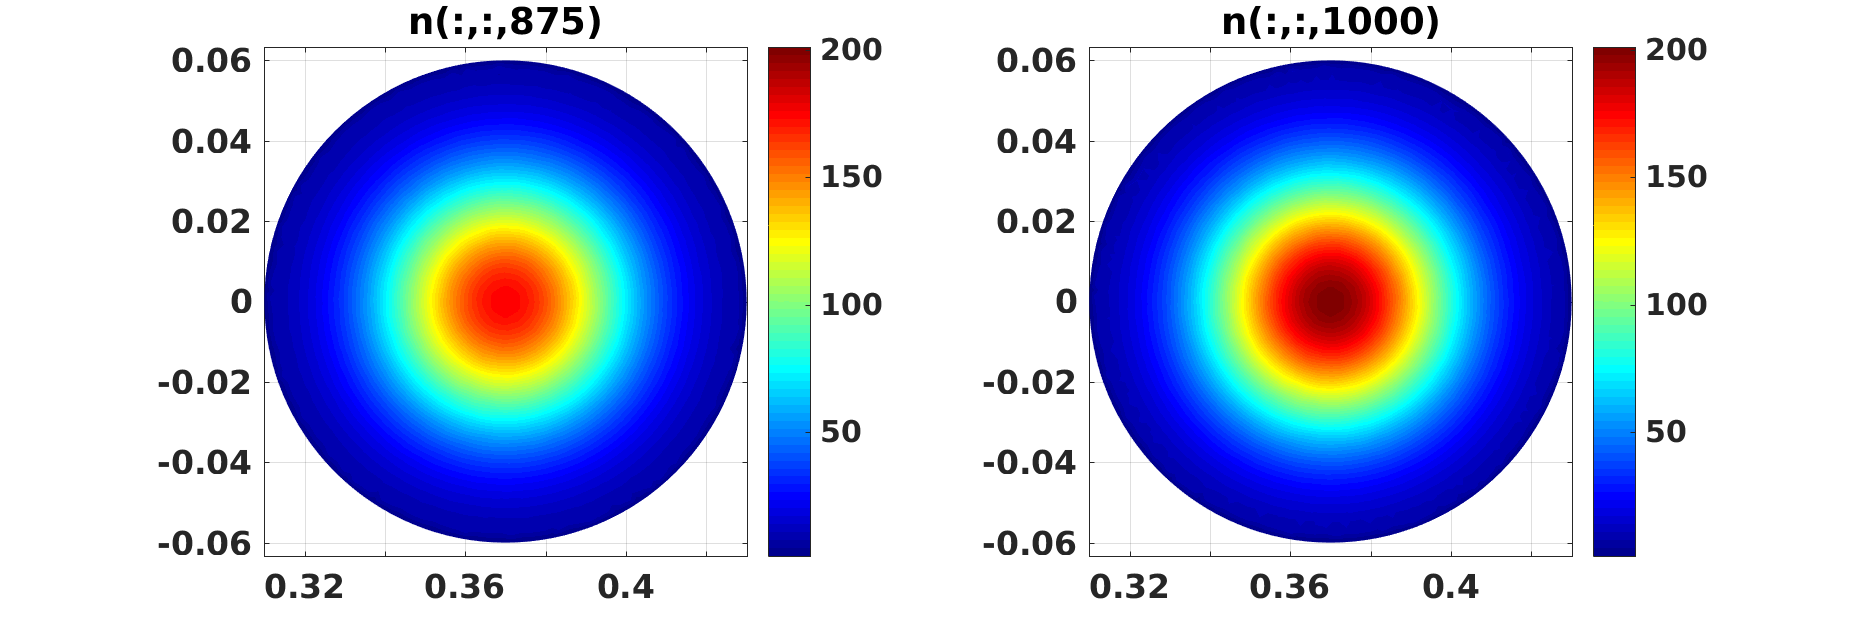
\includegraphics[scale=0.24]{../SImulacao_breakdown/PDE/ntod4B6.png} 
\end{subfigure}
\caption{Densidade de plasma ($m^{-3}$), aproximação da ionização por uma gaussiana ($dt=10^{-5}$\ s, $H_{max} = 0,003$ e $D=0,0002$\ $m^2s^{-1}$).}
\label{densidadeB}
\end{figure}
\end{frame}


\begin{frame}
\frametitle{Aproximação da taxa de ionização menos perda por uma gaussiana}
\begin{figure}[H]
\begin{subfigure}{0.43\textwidth}
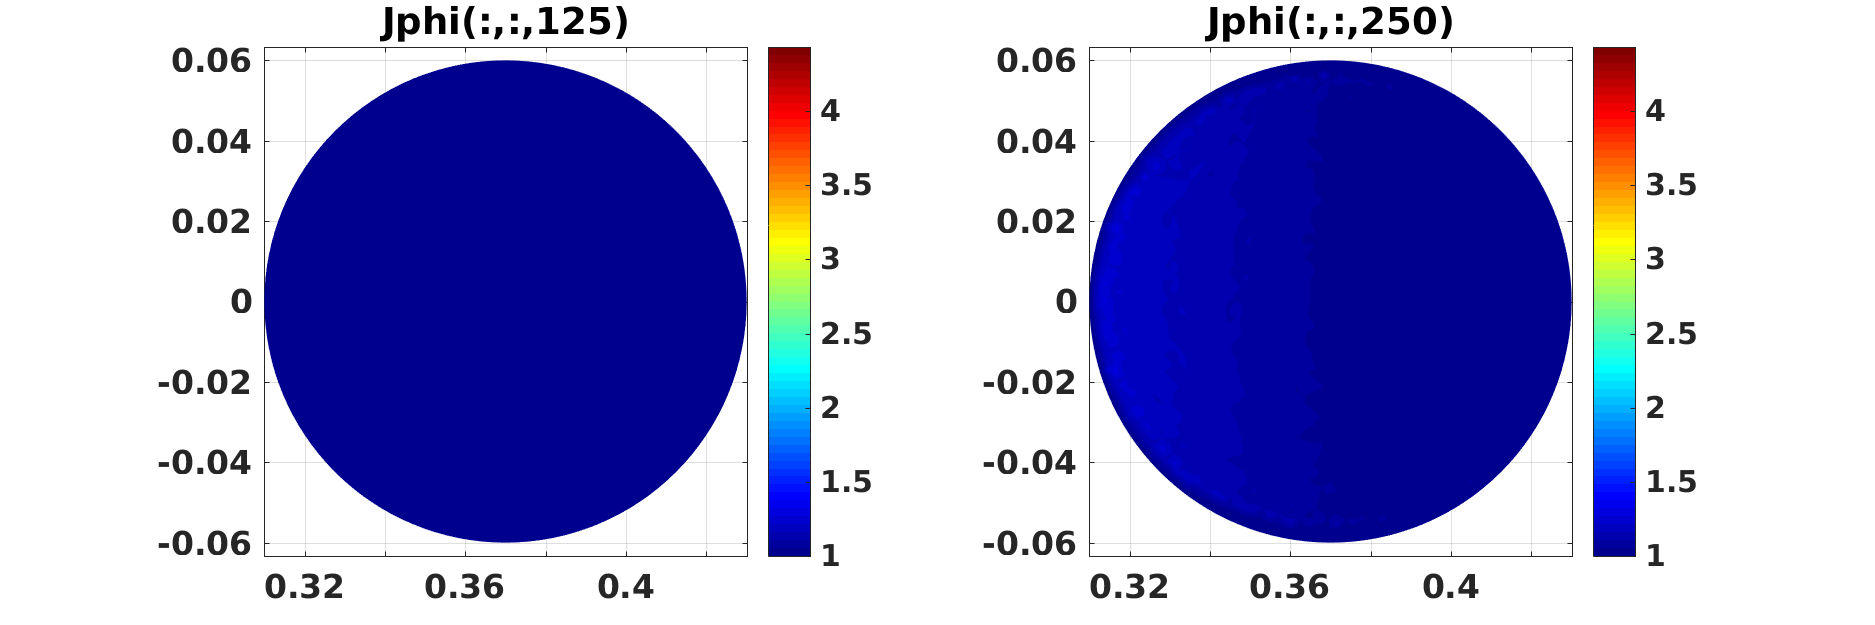
\includegraphics[scale=0.24]{../SImulacao_breakdown/PDE/Jphitod1B6.png}  
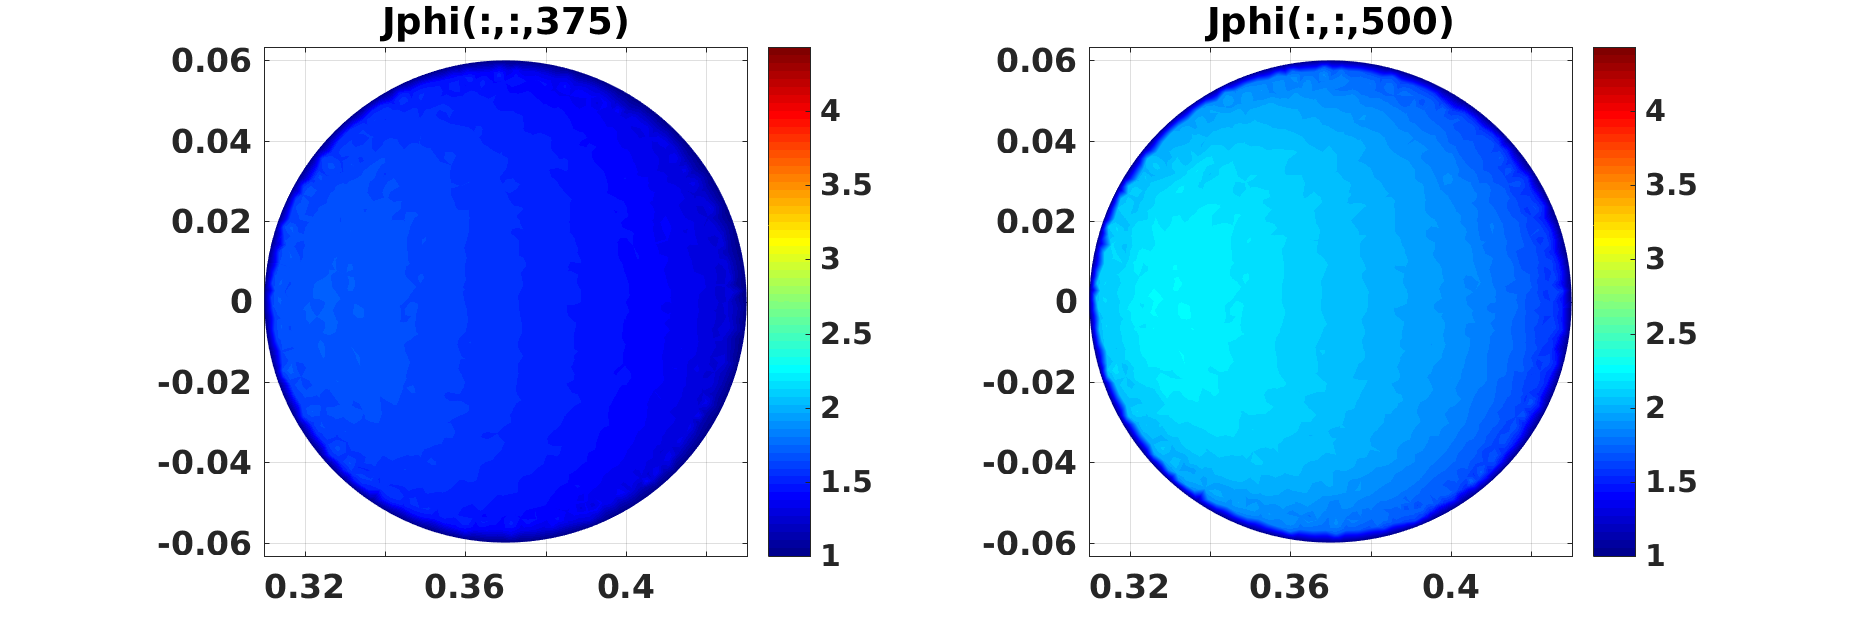
\includegraphics[scale=0.24]{../SImulacao_breakdown/PDE/Jphitod2B6.png} 
\end{subfigure}
\begin{subfigure}{0.43\textwidth}
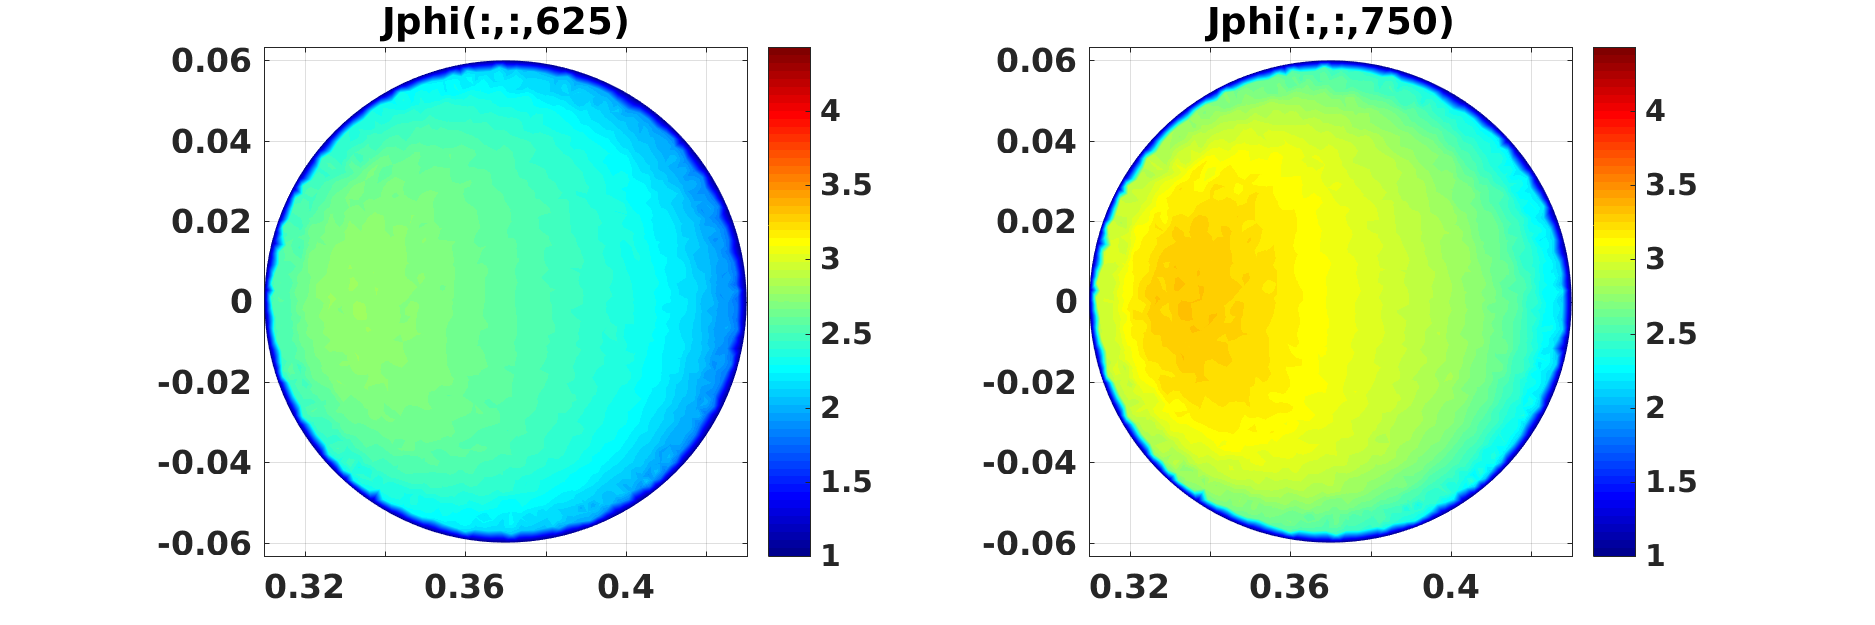
\includegraphics[scale=0.24]{../SImulacao_breakdown/PDE/Jphitod3B6.png} 
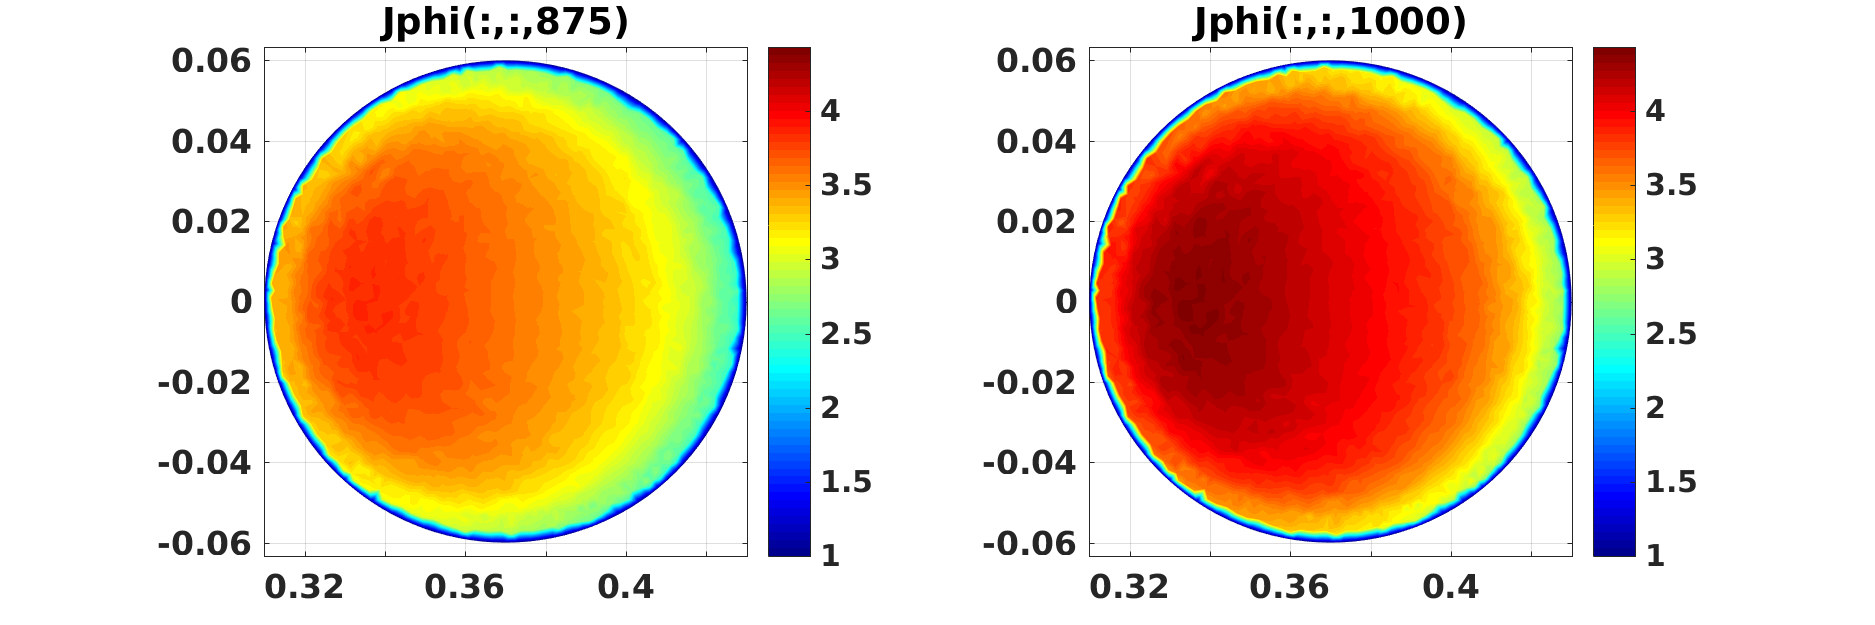
\includegraphics[scale=0.24]{../SImulacao_breakdown/PDE/Jphitod4B6.png} 
\end{subfigure}
\caption{Componente toroidal da densidade de corrente de plasma ($A/m^2$), aproximação da ionização por uma gaussiana. ($dt=10^{-6}$\ s, $H_{max} = 0,003$ e $D=0,0002$\ $m^2s^{-1}$).}
\label{densidadeCB}
\end{figure}
\end{frame}


\begin{frame}
\frametitle{Aproximação da taxa de ionização menos perda por uma gaussiana}
\begin{figure}[H]
\begin{subfigure}{0.43\textwidth}
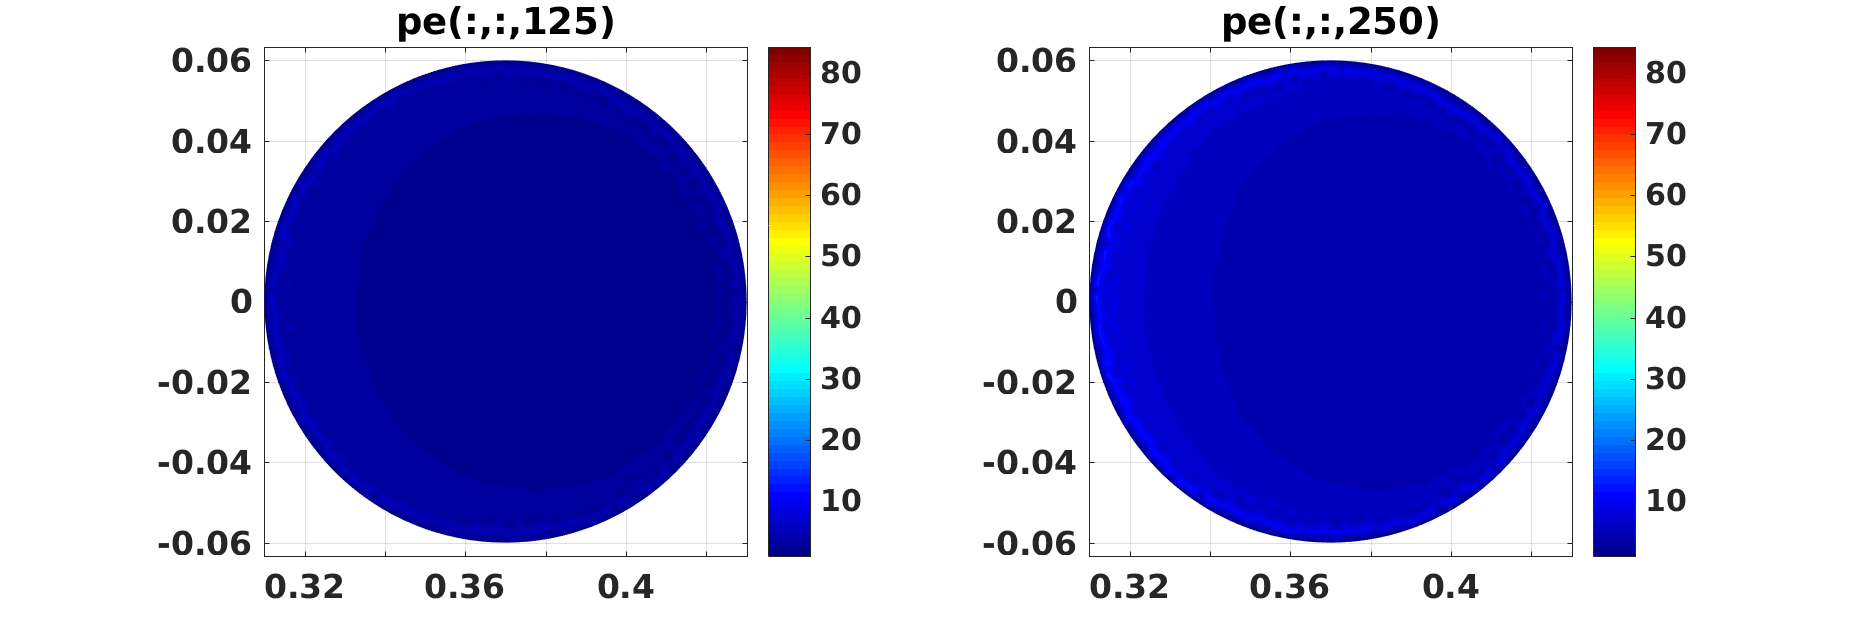
\includegraphics[scale=0.24]{../SImulacao_breakdown/PDE/petod1B6.png}  
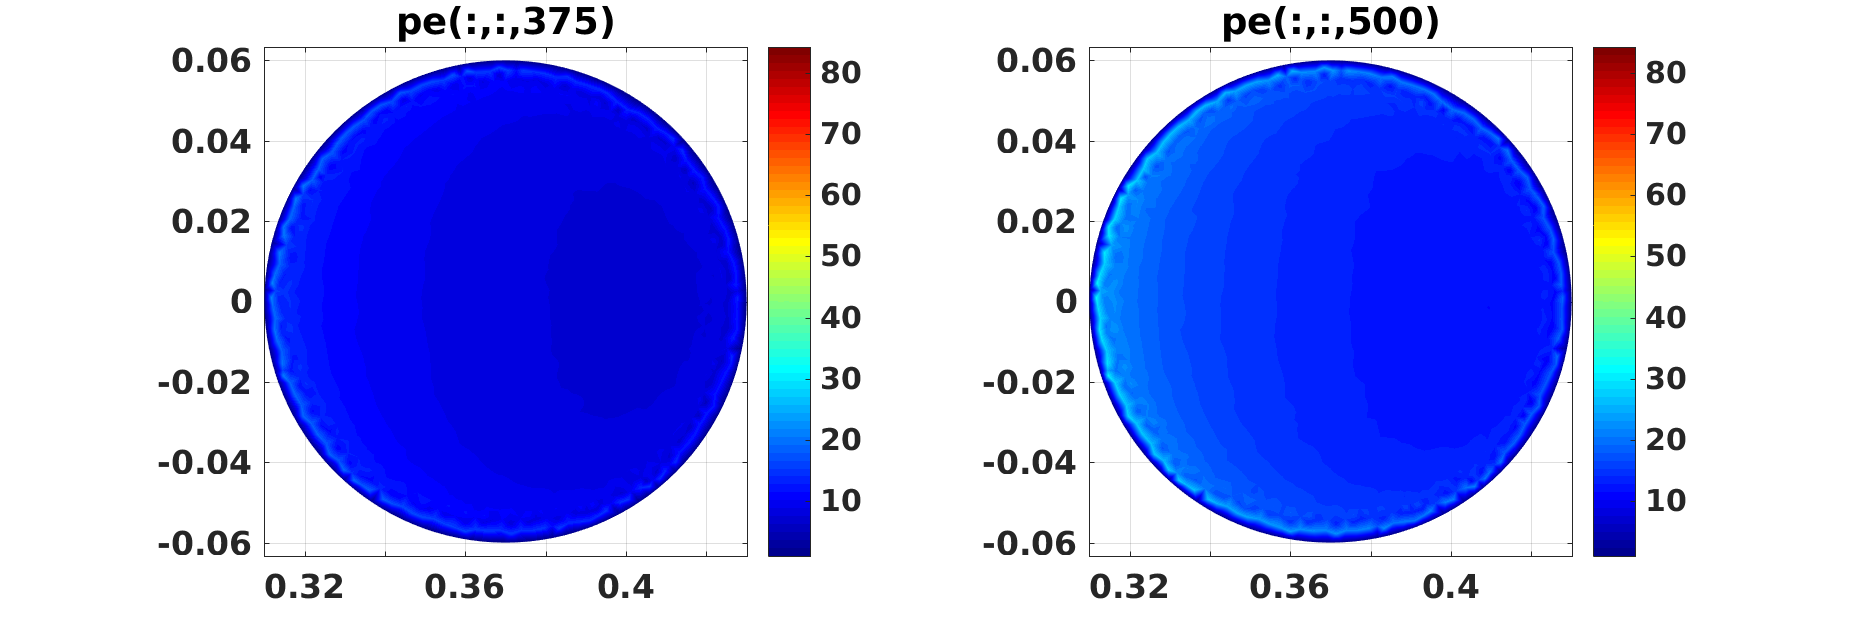
\includegraphics[scale=0.24]{../SImulacao_breakdown/PDE/petod2B6.png} 
\end{subfigure}
\begin{subfigure}{0.43\textwidth}
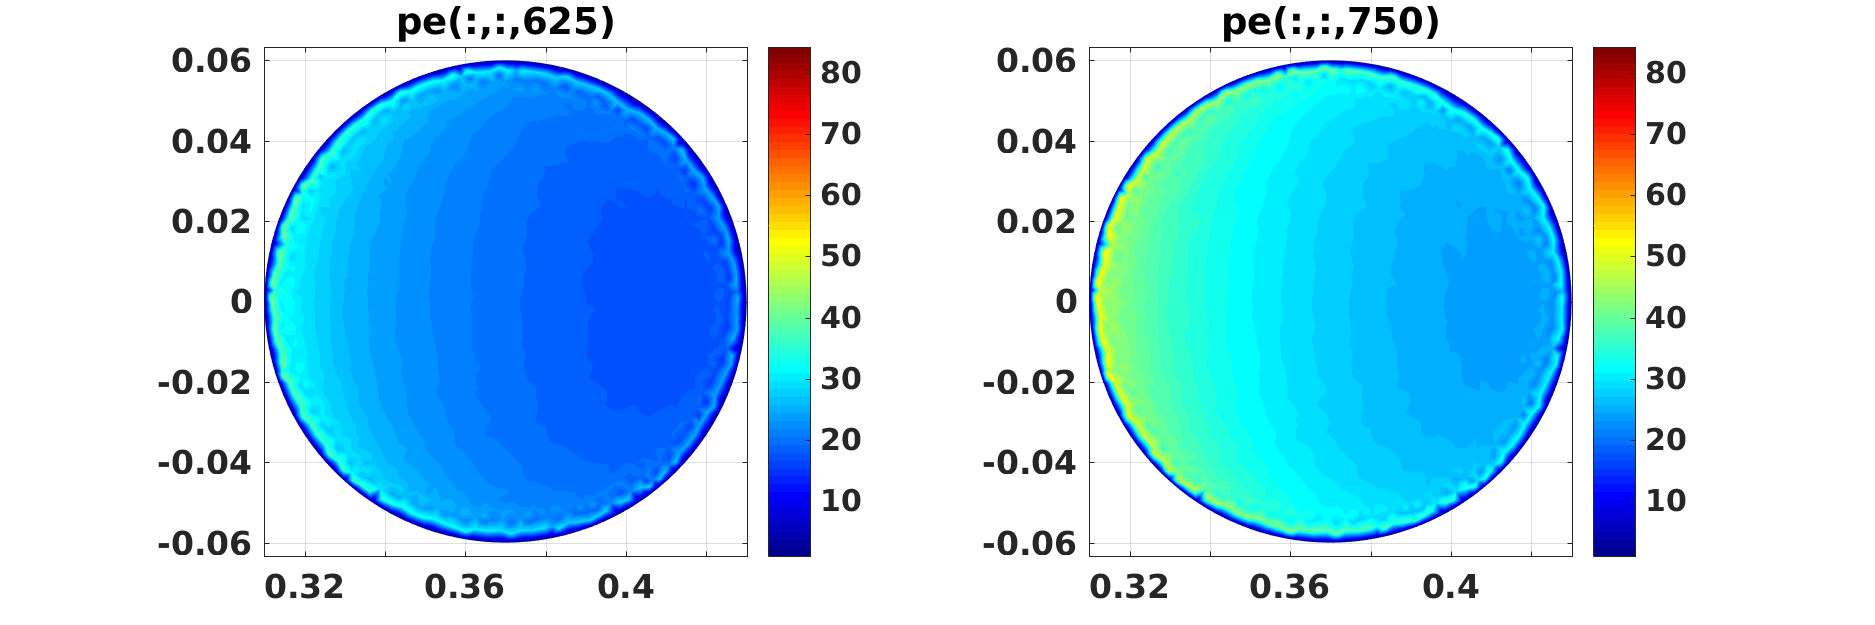
\includegraphics[scale=0.24]{../SImulacao_breakdown/PDE/petod3B6.png} 
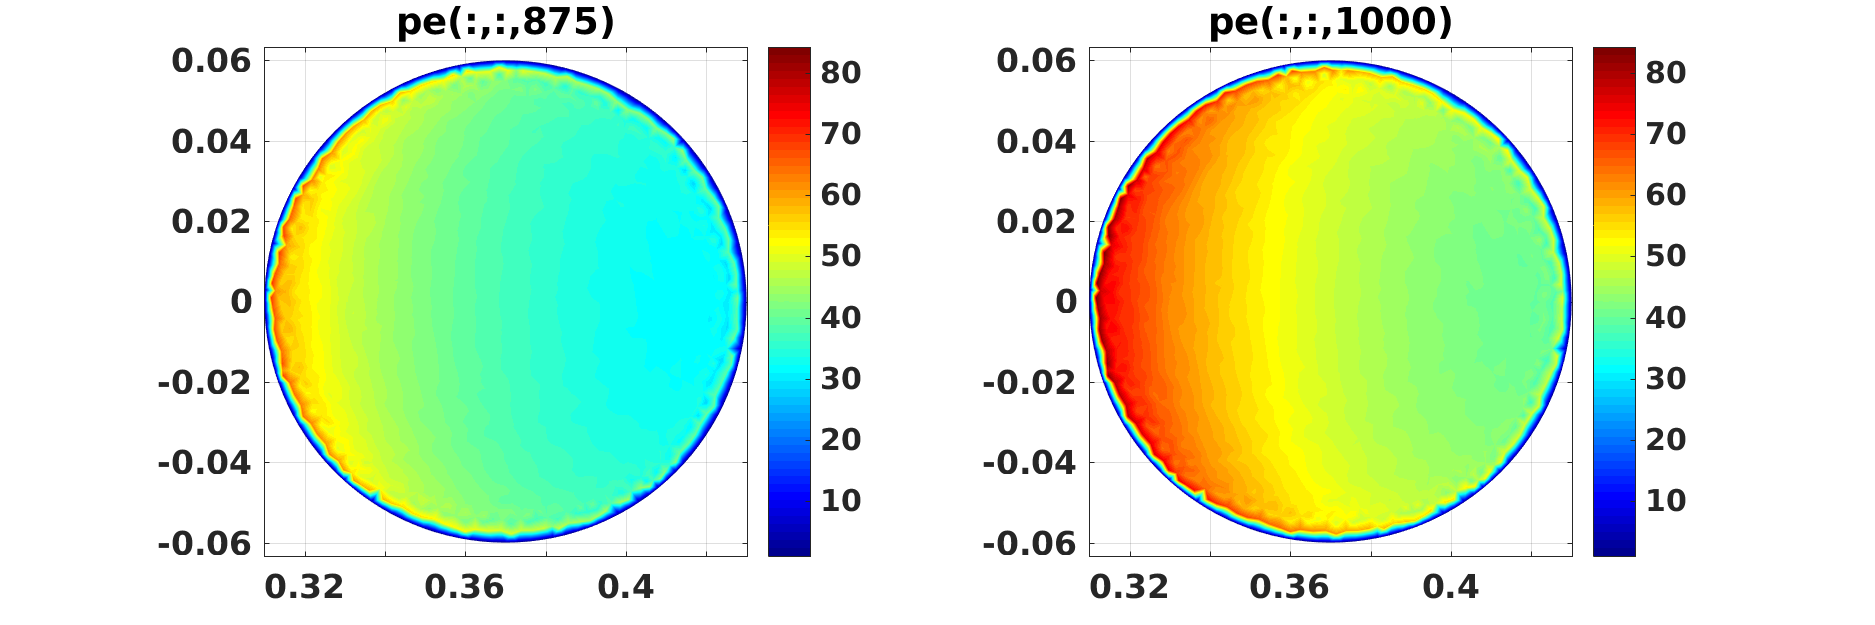
\includegraphics[scale=0.24]{../SImulacao_breakdown/PDE/petod4B6.png} 
\end{subfigure}
\caption{Pressão eletrônica ($Pa$), aproximação da ionização por uma gaussiana ($dt=10^{-5}$\ s, $H_{max} = 0,003$ e $D=0,0002$\ $m^2s^{-1}$).}
\label{pressaoB}
\end{figure}
\end{frame}
\begin{frame}
\frametitle{Aproximação da taxa de ionização menos perda por uma gaussiana}
\begin{figure}[H]
\begin{subfigure}{0.43\textwidth}
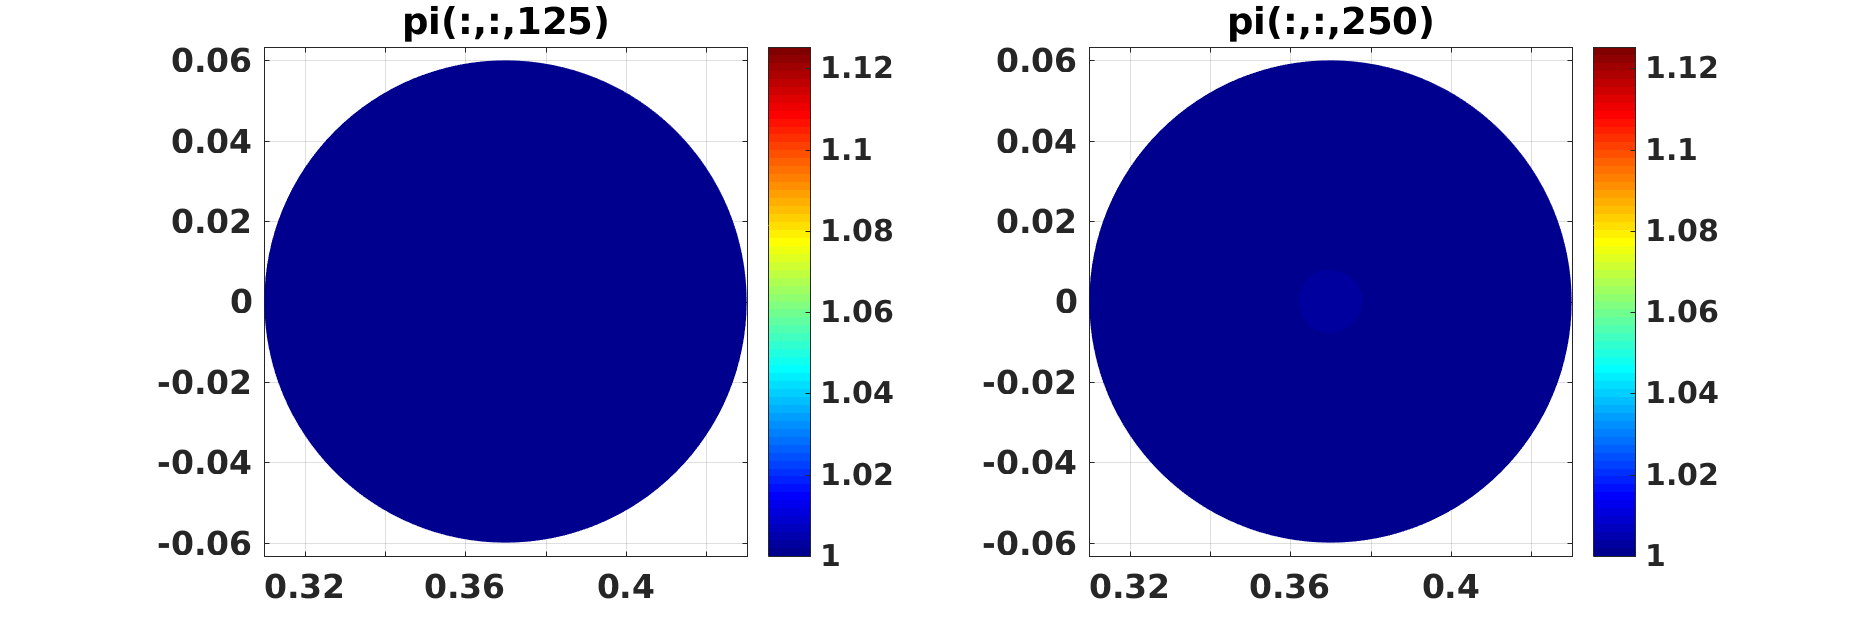
\includegraphics[scale=0.24]{../SImulacao_breakdown/PDE/pitod1B6.png}  
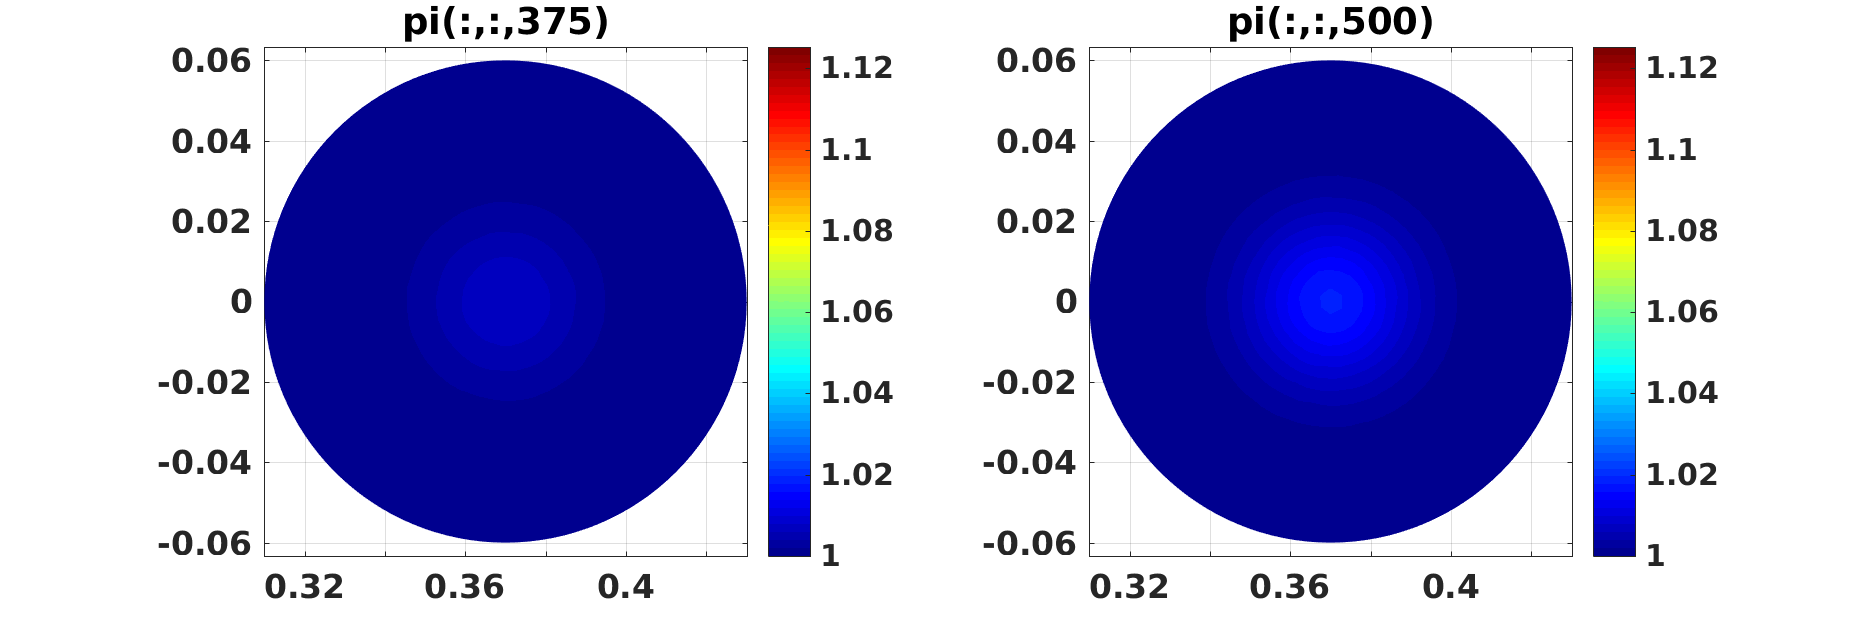
\includegraphics[scale=0.24]{../SImulacao_breakdown/PDE/pitod2B6.png} 
\end{subfigure}
\begin{subfigure}{0.43\textwidth}
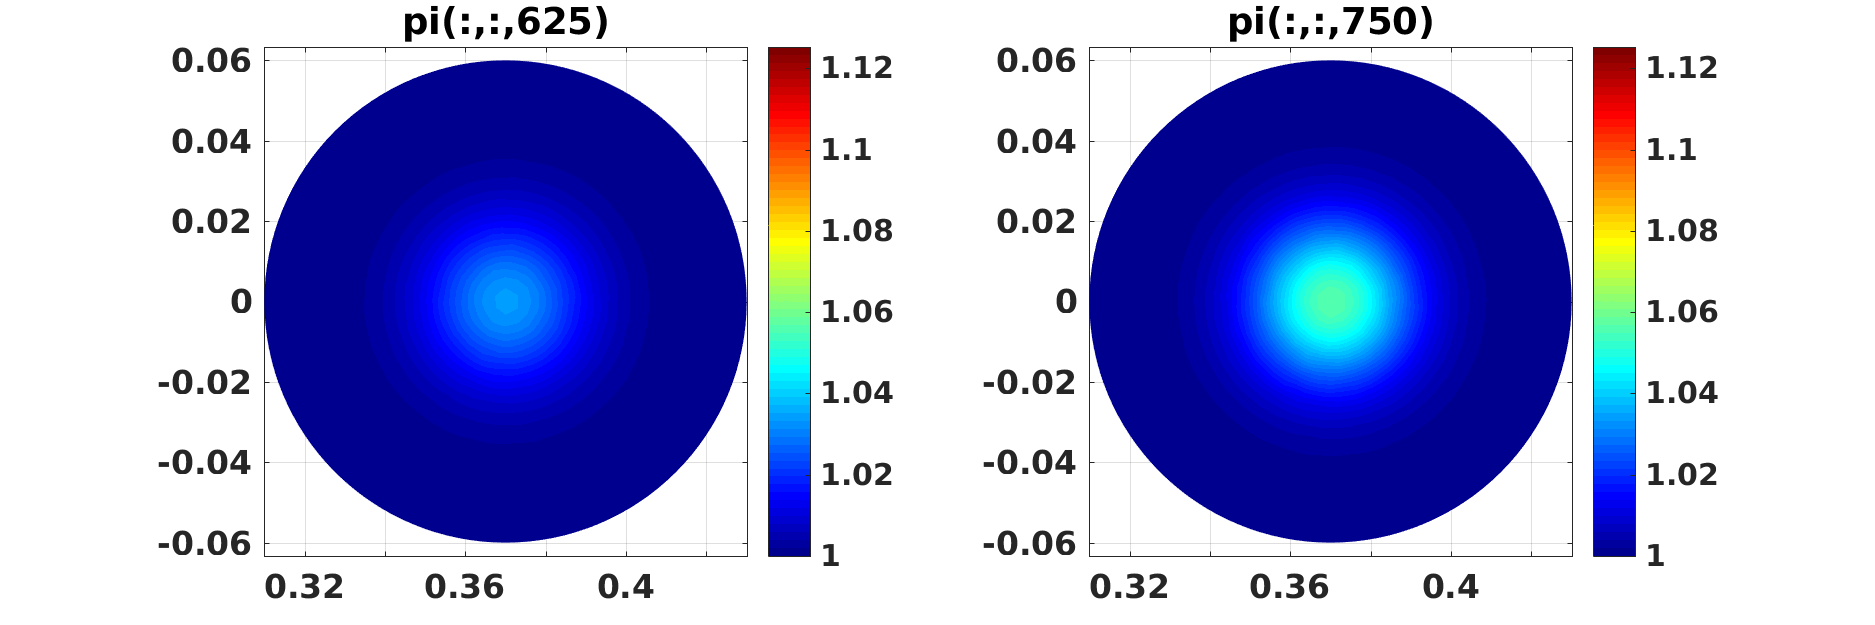
\includegraphics[scale=0.24]{../SImulacao_breakdown/PDE/pitod3B6.png} 
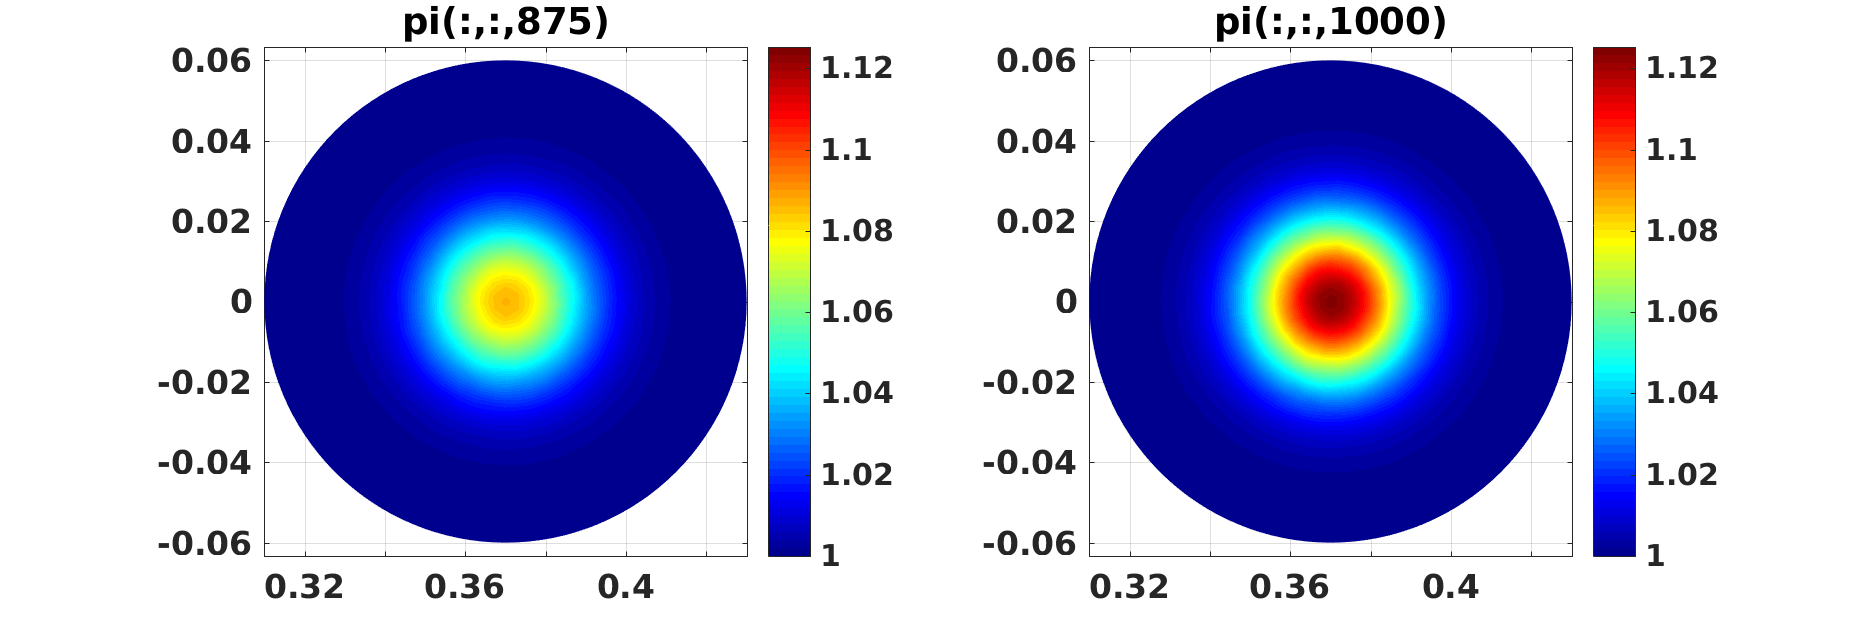
\includegraphics[scale=0.24]{../SImulacao_breakdown/PDE/pitod4B6.png} 
\end{subfigure}
\caption{Pressão iônica ($Pa$), aproximação da ionização por uma gaussiana ($dt=10^{-5}$\ s, $H_{max} = 0,003$ e $D=0,0002$\ $m^2s^{-1}$).}
\end{figure}
\end{frame}

\section{Aproximação da ionização pelo modelo de Townsend}
   \begin{frame}
			\frametitle{Campo elétrico e campo magnético externo}
		\framesubtitle{Malha triangular $H_{max}=0.003$}
\begin{figure}[H]
\begin{center}
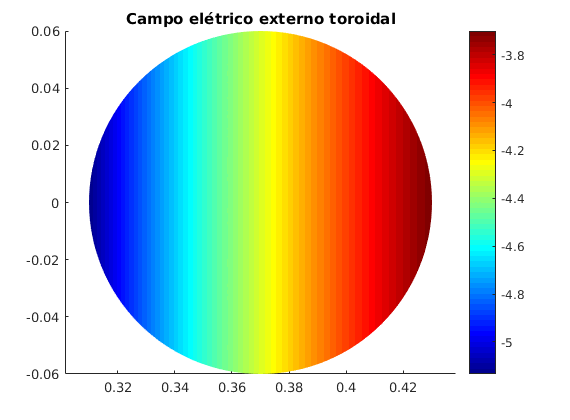
\includegraphics[scale=0.5]{../SImulacao_breakdown/PDE/Campoeleext.png} 
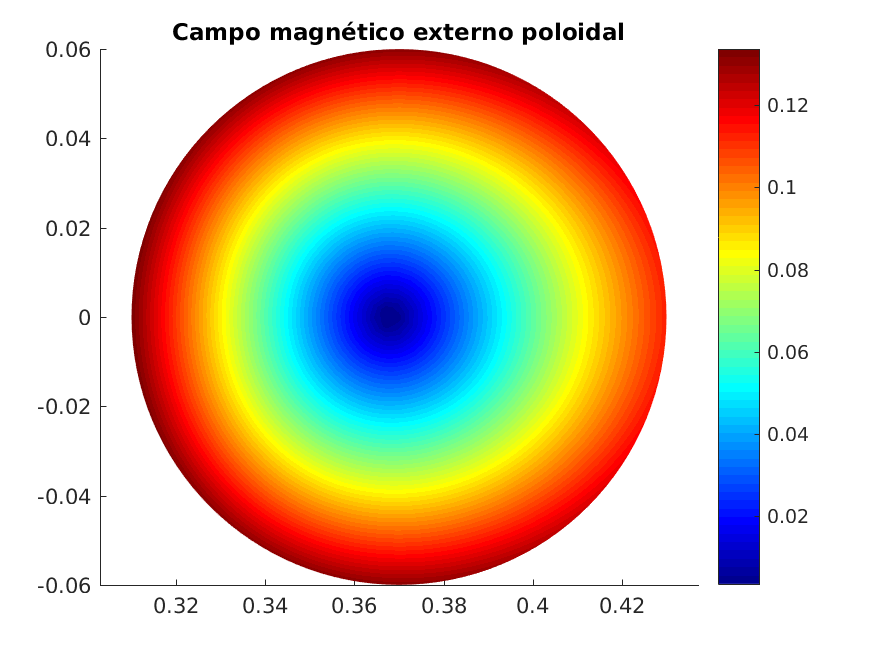
\includegraphics[scale=0.5]{../SImulacao_breakdown/PDE/CampoMagext2.png}
 \caption{Campos elétrico externo toroidal e magnético externo poloidal.}
\end{center}
\end{figure}
\end{frame}	
\begin{frame}
			\frametitle{Campo elétrico e campo magnético externo}
		\framesubtitle{Malha triangular $H_{max}=0.003$}
\begin{figure}[H]
\begin{center}
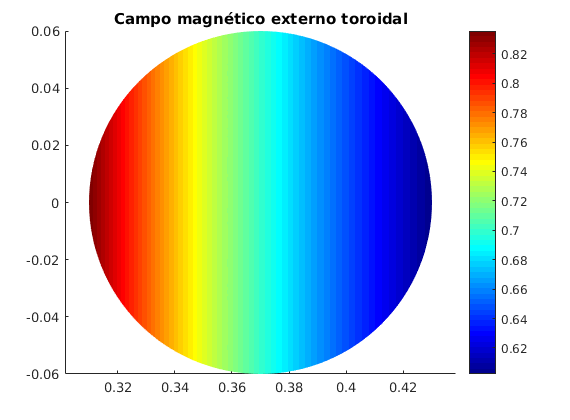
\includegraphics[scale=0.5]{../SImulacao_breakdown/PDE/CampoMagext.png} 
 \caption{Campos magnéticos externo toroidal.}
\end{center}
\end{figure}	
\end{frame}	

	
	\begin{frame}
		\frametitle{PDE Solver: $\nu_{loss}$}
			\begin{figure}[H]
\centering
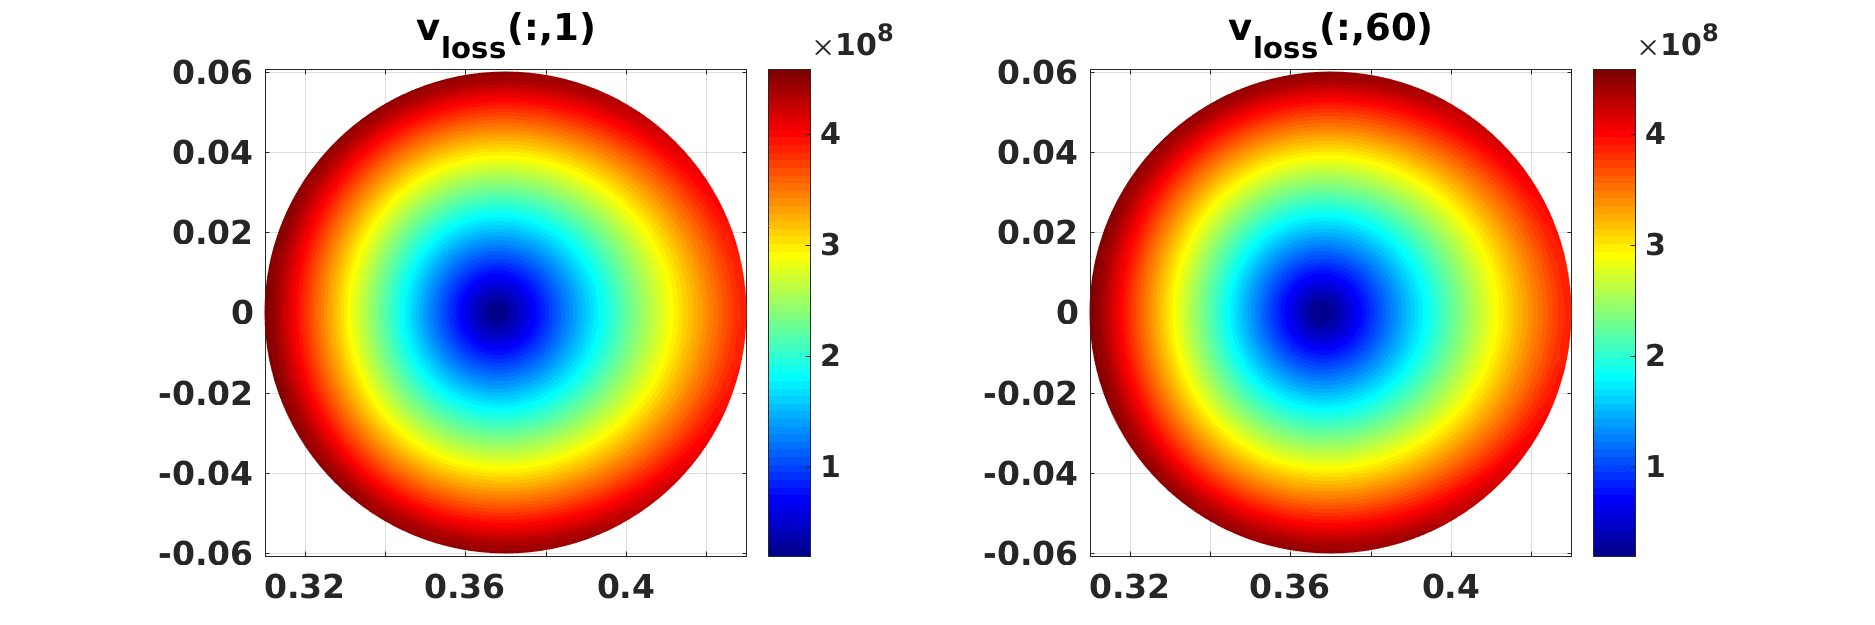
\includegraphics[width=.9\linewidth]{../SImulacao_breakdown/PDE/vinl1.png}  
\caption{Taxa de perda de partículas ($\nu_{loss}$)  ($dt=10e-5$s e $H_{max} = 0.003$).}
\label{vinn1}
\end{figure}
\end{frame}
	
	\begin{frame}
			\frametitle{PDE Solver: $\nu_{in}$}
\begin{figure}[H]
\centering
\includegraphics[width=.9\linewidth]{../SImulacao_breakdown/PDE/vinv1.png}  
\caption{Taxa de ionização $\nu_{in}$ ($s^{-1}$) ($dt=10e-5$s e $H_{max} = 0.003$).}
\label{vinn2}
\end{figure}
\end{frame}
	
	\begin{frame}
			\frametitle{PDE Solver: $\nu_{in}-\nu_{loss}$}
\begin{figure}[H]
\centering
\includegraphics[width=.9\linewidth]{../SImulacao_breakdown/PDE/vinvloss1.png}  
\caption{Taxa de ionização $\nu_{in}$ menos perda de partículas $\nu_{loss}$ ($s^{-1}$) ($dt=10e-5$s e $H_{max} = 0.003$).}
\label{vinn3}
\end{figure}	
	\end{frame}
	
	
			%[width=.7\linewidth]


\begin{frame}		
\frametitle{Aproximação da ionização pelo modelo de Townsend}
Plotagem em termos de proporção, ou seja plotamos o valor da variável macroscópica dividido pela condição inicial.
\begin{figure}[H]
\begin{subfigure}{0.43\textwidth}
\includegraphics[scale=0.24]{../SImulacao_breakdown/PDE/ntod1B2.png}  
\includegraphics[scale=0.24]{../SImulacao_breakdown/PDE/ntod2B2.png}
\end{subfigure}
\begin{subfigure}{0.43\textwidth}
\includegraphics[scale=0.24]{../SImulacao_breakdown/PDE/ntod3B2.png} 
\includegraphics[scale=0.24]{../SImulacao_breakdown/PDE/ntod4B2.png}
\end{subfigure}	
\caption{Densidade de plasma ($m^{-3}$), fonte de partículas modelada através do modelo de Townsend ($dt=10^{-5}$\ s, $H_{max} = 0,003$ e $D=0,0002$\ $m^2s^{-1}$).}
\end{figure}
\end{frame}
	
	\begin{frame}		
\frametitle{Aproximação da ionização pelo modelo de Townsend}

\begin{figure}[H]
\begin{subfigure}{0.43\textwidth}
\includegraphics[scale=0.24]{../SImulacao_breakdown/PDE/Jphitod1B2.png}  
\includegraphics[scale=0.24]{../SImulacao_breakdown/PDE/Jphitod2B2.png} 
\end{subfigure}
\begin{subfigure}{0.43\textwidth}
\includegraphics[scale=0.24]{../SImulacao_breakdown/PDE/Jphitod3B2.png} 
\includegraphics[scale=0.24]{../SImulacao_breakdown/PDE/Jphitod4B2.png} 
\end{subfigure}	
\caption{Componente toroidal da densidade de corrente de plasma ($A/m^2$), fonte de partículas modelada através do modelo de Townsend ($dt=10^{-5}$\ s, $H_{max} = 0,003$ e $D=0,0002$\ $m^2s^{-1}$).}
\end{figure}
\end{frame}


\begin{frame}		
\frametitle{Aproximação da ionização pelo modelo de Townsend}
\begin{figure}[H]
\begin{subfigure}{0.43\textwidth}
\includegraphics[scale=0.24]{../SImulacao_breakdown/PDE/petod1B2.png}  
\includegraphics[scale=0.24]{../SImulacao_breakdown/PDE/petod2B2.png} 
\end{subfigure}
\begin{subfigure}{0.43\textwidth}
\includegraphics[scale=0.24]{../SImulacao_breakdown/PDE/petod3B2.png} 
\includegraphics[scale=0.24]{../SImulacao_breakdown/PDE/petod4B2.png}
\end{subfigure}	
\caption{Pressão eletrônica ($Pa$), fonte de partículas modelada através do modelo de Townsend ($dt=10^{-5}$\ s, $H_{max} = 0,003$ e $D=0,0002$\ $m^2s^{-1}$).}
\end{figure}
\end{frame}


\begin{frame}		
\frametitle{Aproximação da ionização pelo modelo de Townsend}
%\framesubtitle{ ss }
\begin{figure}[H]
\begin{subfigure}{0.43\textwidth}
\includegraphics[scale=0.24]{../SImulacao_breakdown/PDE/pitod1B2.png}  
\includegraphics[scale=0.24]{../SImulacao_breakdown/PDE/pitod2B2.png} 
\end{subfigure}
\begin{subfigure}{0.43\textwidth}
\includegraphics[scale=0.24]{../SImulacao_breakdown/PDE/pitod3B2.png} 
\includegraphics[scale=0.24]{../SImulacao_breakdown/PDE/pitod4B2.png} 
\end{subfigure}	
\caption{Pressão iônica ($Pa$), fonte de partículas modelada através do modelo de Townsend ($dt=10^{-5}$\ s, $H_{max} = 0,003$ e $D=0,0002$\ $m^2s^{-1}$).}
\end{figure}
\end{frame}

\section{Aproximação do campo magnético gerado pelo plasma}
%Resultados com os coeficientes de transporte
\begin{frame}		
\frametitle{ Aproximação do campo magnético gerado pelo plasma}
 Nesta simulação temos simultaneamente ativados a aproximação pela gaussiana com $s_0=10^{11}$, $x_0=0$ e $\sigma=0.001$ e também a taxa de criação $\nu_{in}$ e perda $ \nu_{loss}$ de partículas obtidas através do modelo de Townsend.
\end{frame}

\begin{frame}		
\frametitle{Aproximação do campo magnético gerado pelo plasma }

Com $D=0$ temos
\begin{figure}[H]
\begin{subfigure}{0.43\textwidth}
\includegraphics[scale=0.24]{../SImulacao_breakdown/PDE/ntod1B3.png}  
\includegraphics[scale=0.24]{../SImulacao_breakdown/PDE/ntod2B3.png}
\end{subfigure}
\begin{subfigure}{0.43\textwidth}
\includegraphics[scale=0.24]{../SImulacao_breakdown/PDE/ntod3B3.png} 
\includegraphics[scale=0.24]{../SImulacao_breakdown/PDE/ntod4B3.png} 
\end{subfigure}
\caption{Densidade de plasma ($m^{-3}$), fonte de partículas modelada através do modelo de Townsend ($dt=10^{-5}$\ s, $H_{max} = 0,003$ e $D=0$\ $m^2s^{-1}$).}
\label{campplasmasil1}
\end{figure}
\end{frame}

\begin{frame}		
\frametitle{ Aproximação do campo magnético gerado pelo plasma}
\begin{figure}[H]
\begin{subfigure}{0.43\textwidth}
\includegraphics[scale=0.24]{../SImulacao_breakdown/PDE/Jphitod1B3.png}  
\includegraphics[scale=0.24]{../SImulacao_breakdown/PDE/Jphitod2B3.png}
\end{subfigure}
\begin{subfigure}{0.43\textwidth}
\includegraphics[scale=0.24]{../SImulacao_breakdown/PDE/Jphitod3B3.png} 
\includegraphics[scale=0.24]{../SImulacao_breakdown/PDE/Jphitod4B3.png} 
\end{subfigure}
\caption{Componente toroidal da densidade de corrente de plasma ($A/m^2$), fonte de partículas modelada através do modelo de Townsend ($dt=10^{-5}$\ s, $H_{max} = 0,003$ e $D=0$\ $m^2s^{-1}$).}
\label{campplasmasil2}
\end{figure}
\end{frame}


\begin{frame}	
\frametitle{ Aproximação do campo magnético gerado pelo plasma}
\begin{figure}[H]
\begin{subfigure}{0.43\textwidth}
\includegraphics[scale=0.24]{../SImulacao_breakdown/PDE/petod1B3.png}  
\includegraphics[scale=0.24]{../SImulacao_breakdown/PDE/petod2B3.png}
\end{subfigure}
\begin{subfigure}{0.43\textwidth}
\includegraphics[scale=0.24]{../SImulacao_breakdown/PDE/petod3B3.png} 
\includegraphics[scale=0.24]{../SImulacao_breakdown/PDE/petod4B3.png}
\end{subfigure}	
\caption{Pressão eletrônica ($Pa$), fonte de partículas modelada através do modelo de Townsend ($dt=10^{-5}$\ s, $H_{max} = 0,003$ e $D=0$\ $m^2s^{-1}$).}
\label{campplasmasil3}
\end{figure}
\end{frame}


\begin{frame}		
\frametitle{ Aproximação do campo magnético gerado pelo plasma}
\begin{figure}[H]
\begin{subfigure}{0.43\textwidth}
\includegraphics[scale=0.24]{../SImulacao_breakdown/PDE/pitod1B3.png}  
\includegraphics[scale=0.24]{../SImulacao_breakdown/PDE/pitod2B3.png} 
\end{subfigure}
\begin{subfigure}{0.43\textwidth}
\includegraphics[scale=0.24]{../SImulacao_breakdown/PDE/pitod3B3.png} 
\includegraphics[scale=0.24]{../SImulacao_breakdown/PDE/pitod4B3.png} 
\end{subfigure}
\caption{Pressão iônica ($Pa$), aproximação da ionização por uma gaussiana ($dt=10^{-5}$\ s, $H_{max} = 0,003$ e $D=0$\ $m^2s^{-1}$).}
\end{figure}

\end{frame}




\section{Conclusão}


  %Na figura \ref{temperaturaB} nota-se que na distribuição da temperatura dos elétrons os maiores valores coincidem com os maiores valores da densidade de corrente toroidal. Pode-se concluir também que  $T_e+T_i \approx T_e = T_{e,i}$, uma vez que a temperatura de elétrons na fase inicial é maior que a temperatura dos íons.   

%O código usando o PDE Solver é bem completo, permite a troca entre a aproximação pela gaussiana e a volta para os coeficientes calculados através dos campos magnéticos e elétricos externos apenas alternando o valor de uma variável de controle. Também pode-se ativar o campo magnético gerado pelo plasma por meio de uma variável de controle. Permite ativar a plotagem das quatro distribuições ao longo do tempo $n, J_\phi, p_e, p_i$ para qualquer conjunto de tempos, apenas alterando o valor de uma variável de controle na estrutura G, que é uma estrutura global, importada em todos as sub-rotinas chamadas ao longo da execução. A estrutura G contêm todos os dados de controle além das distribuições de campos e quaisquer dados que precisem ser mantidos para reutilização ao longo da execução do código. Além de permitir a ativação da plotagem de animações no tempo para qualquer uma das distribuições das variáveis macroscópicas e para os valores de $\nu_{en}$, $\nu_{loss}$, $\nu_{in}$, $\nu_{en}$, $\eta$.

%Uma adaptação do código explícito no tempo se faz necessária uma vez que atualmente no PDE solver não é possível diminuir o $dt$ e aumentar o valor de $D$ sem o tempo de processamento explodir. Portanto  Para isso pretende-se usar uma malha triangular adaptativa, ou alguns subdomínios, no código explícito no tempo para resolver o sistema nesta malha, pois no ponto de zero campo magnético é necessário uma malha muito mais refinada do que ao longo da fronteira do domínio circular. 


   \begin{frame}
			\frametitle{Conclusão}
		\begin{itemize}
			 \item Resultados coerentes com o esperado do modelo. 
			 \item Campos elétrico e magnético coerentes com os campos reais.%e gerando uma distribuição de componente toroidal da densidade de corrente de plasma ($A/m^2$), que decai proporcionalmente ao campo elétrico conforme o raio em relação ao centro da câmera de vácuo do tokamak aumenta. 
			 \item Resultados da abordagem explícita enfrentam   problemas numéricos como os coeficientes de transporte aumentarem abruptamente após alguns intervalos de tempo.   
              
		\end{itemize}

	\end{frame}	
	  \begin{frame}
			\frametitle{Conclusão}
		\begin{itemize}
			 \item  Pela abordagem do PDE solver as condições de contorno foram aplicadas de maneira auto consistente. 
			 \item Os resultados obtidos foram mais consistentes que os obtidos na abordagem explícita. 
			 \item Os coeficientes de transporte se mantiveram dentro da faixa esperada. %sem sofrer os aumentos assintóticos que vimos nos coeficientes de transporte no código explícito.

              
		\end{itemize}

	\end{frame}	
	

	\begin{frame}		
			\frametitle{Conclusão}
\begin{itemize}
			 \item A densidade numérica de partículas no plasma inicial aumenta junto da componente toroidal da densidade de corrente de plasma  
			 \item Tendo uma concentração maior justamente no ponto de zero campo magnético onde o confinamento é mais eficiente. 
			 \item A pressão eletrônica tem seus maiores valores onde o campo elétrico externo é mais forte. 
			 \item Também foi mais afetada pelo aumento da densidade de partículas do que a pressão iônica. 
\end{itemize}
\end{frame}


	
	
	  \begin{frame}
			\frametitle{Conclusão}
		\begin{itemize}
			 \item  Nas simulações modelando a criação $\nu_{in}$ e perda $ \nu_{loss}$ de partículas através do modelo de Townsend vimos uma mudança na quantidade $\nu_{in}-\nu_{loss}$ com relação a gaussiana, uma vez que $\nu_{in}$ ficou dependente do campo elétrico figura \ref{vinn1} e $ \nu_{loss}$ tem seu menor valor no ponto de zero campo magnético figura \ref{vinn2}. 
			 \item Da figura \ref{vinn3} vemos que é perfeitamente viável aproximar $\nu_{in}-\nu_{loss}$ por uma gaussiana como na figura \ref{grafgaussiana}. 

		\end{itemize}

	\end{frame}	
	  \begin{frame}
			\frametitle{Conclusão}
		\begin{itemize}
					 \item Nas simulações deste trabalho a diferença $\nu_{in}-\nu_{loss}$ se mantém praticamente constante durante a  simulação.
              \item  Adicionando o campo magnético gerado pelo plasma foi visto uma melhora no confinamento. 
              \item Nas continuação deste trabalho pretende-se implementar de maneira auto-consistente as equações dos campos gerados pelo plasma.
			 \item  A continuação deste trabalho buscará usar o melhor das duas abordagens, explícita no tempo e pelo PDE solver. 
              \item Obter um código mais flexível que permitirá obter resultados mais precisos.
		\end{itemize}

	\end{frame}	

\section{Refer\^{e}ncias bibliogr\'{a}ficas}

\begin{frame}
		%[allowframebreaks]
		\frametitle{Refer\^{e}ncias bibliogr\'{a}ficas}
		
		
		
		
		\bibliography{TCC_2}
	\end{frame}

\end{document}
